\documentclass[ASNA,twocolumn]{USG} %twocolumn
\usepackage{anyfontsize} %

\usepackage{colortbl}   % For coloring table lines
\usepackage{xcolor}     % For color definitions

\usepackage{steinmetz}
\graphicspath{{./images/}}

\articletype{ORIGINAL ARTICLE}%
\subarticletype{}

\received{}
\revised{}
\accepted{}
\journal{Expert Systems}
\volume{0}
\copyyear{2026}
\startpage{1}
\articledoi{10.1002/0000}

%\raggedbottom

%%
%\renewcommand\ShowFrameLinethickness{0.15pt}
%\renewcommand*\ShowFrameColor{\color{red}}


\begin{document}

\title{KSRA: Identifying kernelized self-representation anomalies}
%\subtitle{Subtitle}
\author[1]{Zhong Yuan}[https://orcid.org/0000-0002-7456-4445]
\author[1]{Luoshu Yang}[https://orcid.org/0009-0007-4225-5289]
\author[1]{Xinyu Su}[https://orcid.org/0009-0001-1092-2426]
\author[2]{Yun-Cheng Liu}[yuncheng.liu@swun.edu.cn]
\author[3]{Yeshalem Gezahegn}[contactyeshalem@dbu.edu.et]
\author[4]{Yingke Chen}[yingke.chen@northumbria.ac.uk]
\author[1]{Dezhong Peng}[pengdz@scu.edu.cn]

\address[1]{College of Computer Science, Sichuan University, Chengdu 610065, China}

\address[2]{School of Mathematics, Southwest Minzu University, Chengdu 610041, China}

\address[3]{College of Computing Science, Debre Berhan University,445 Debre Berhan, Ethiopia}

\address[4]{Department of Computer and Information Sciences, Northumbria University, Newcastle upon Tyne NE1 8ST, UK}

\corres{Zhong Yuan  (\email{yuanzhong@scu.edu.cn}) }

\editor{\textbf{Academic Editor:}  ~|~ \textbf{Guest Editor:} }

\fundingInfo{National Natural Science Foundation of China Number: 62306196 and 12501439; Sichuan Science and Technology Program Number: 2026NSFSC0783.}

\keywords{Anomaly detection | Outlier detection | Kernel function | Self-representation | Mixed data}

\abstract[ABSTRACT]{
Anomaly detection is a pivotal technology in fields such as data mining, information security, and image processing. Existing research, however, faces two major challenges: 1) traditional proximity-based detection methods are susceptible to the distance concentration effect in high-dimensional spaces, leading to a decline in detection performance. 2) most models are only compatible with single-attribute data (either numerical or nominal), making them struggle with the mixed-type data prevalent in real-world scenarios, which limits their applicability. To address these challenges, this paper proposes a Kernelized Self-Representation-based Anomaly detection (KSRA) method, an anomaly detection method that uses a mixed kernel to construct nonlinear similarity profiles from numerical and categorical attributes. These profiles provide a unified representation for subsequent self-representation learning. Building upon this, a generalized kernel self-representation framework is constructed. Four model variants are systematically derived based on different combinations of loss and regularization terms. A random walk on the learned graph produces a structural anomaly score, which is combined with a kernel-derived isolation weight to score each sample. On 20 benchmark datasets, the fixed variant KSRA$_2$ achieved the highest mean ROC-AUC among the fixed methods in the main comparison under the reported tuning protocol.

The source code is publicly available at \url{https://github.com/LsHyrN/KSRA}.
}

\abbr{5-FU, 5-fluorouracil; CFD, computational fluid dynamics; CH, channel; EFS, event-free survival; GBM, glioblastoma multiforme; OS, overall survival; PFS, progression-free
survival; SD, standard deviation.}

\contributed{Hao Zhang and Pengyue D. Guo contributed equally to this study.}

\dedicated{Dedicated to Srivivasa Ramanujano on the occasion of his 125th birth anniversary.}

\copyright{This is an open access article under the terms of the \href{Creative Commons Attribution-NonCommercial}{Creative Commons Attribution-NonCommercial} License, which permits use, distribution and reproduction in any medium, provided the
original~work~is~properly cited and is not used for commercial purposes.
%\\[5pt]
%  ©  2024 The Author(s) \textit{AIChE Journal} published by Wiley Periodicals LLC on behalf of American Institute of Chemical Engineers.
}

%\openaccessstatement

\maketitle
%\afterpage{\aftergroup\restoregeometry}

%\onecolumn

\section{Introduction}\label{Introduction}

Outlier detection (also known as anomaly detection) identifies samples deviating from normal patterns, playing a vital role in network intrusion, fraud detection, and image/video analysis \cite{choras2012statistical, hilal2022financial, pei2024robust, shaik2025leveraging}. These practical tasks usually require higher performance of outlier detection algorithms, so further exploration of effective outlier detection models is of great theoretical and applied significance.

In recent years, the academic community has proposed a variety of anomaly detection algorithms. Typical detection techniques can be broadly categorized into the following types: statistical-based, proximity-based, and clustering-based methods \cite{smiti2020critical}.
Among these, statistical-based methods typically rely on predefined probability distribution models to identify anomalies by detecting samples that deviate significantly from the standard distribution. Such methods often incur high computational costs when dealing with data of unknown distribution or high-dimensional or large-scale datasets. Clustering-based methods, on the other hand, identify outliers by partitioning data into cluster structures, regarding samples that do not fit into any cluster or reside far from cluster centers as anomalies. Nevertheless, their performance is heavily constrained by complex parameter configurations, and the algorithms themselves are inherently sensitive to noise and outliers.

Proximity-based methods primarily fall into two categories: distance-based and density-based. These methods are independent of data distribution and easy to implement; they either identify outliers lacking sufficient neighbors by calculating global distances, or detect anomalous samples that do not conform to the characteristics of their neighborhoods by measuring local density. Although these methods differ in their theoretical approaches, the mainstream proximity-based techniques are, in essence, highly dependent on measures of proximity between samples.
To be more specific, these methods often use explicit metrics, such as Euclidean distance, to assess the degree of deviation of samples \cite {mandhare2017comparative}. Increasing irrelevant dimensionality can reduce relative differences among sample distances, potentially weakening proximity-based anomaly discrimination. This motivates examining representations that retain useful structural distinctions under such conditions.


To address the potential loss of distance discrimination in high-dimensional spaces, representation learning-based methods have received increasing attention. For example, Zhao et al. \cite{zhao2018xgbod} use unsupervised algorithms to extract feature representations to enhance the discriminative power of supervised classifiers; Pang et al. \cite{pang2018learning} achieve stable detection in ultra-high-dimensional data by integrating representation learning with stochastic distance metrics; while Su et al. \cite{su2026outlier} address data uncertainty by combining fuzzy information granulation with representation learning. 

Among the numerous representation learning paradigms, self-representation techniques stand out for their ability to directly capture the collaborative relationships among samples \cite{quan2025class}. Rather than relying solely on predefined Euclidean distances, these techniques learn latent correlations among samples directly from the data features by seeking sparse or low-rank linear representation structures. By virtue of their ability to capture the intrinsic topological structure of data through learned global reconstruction coefficients, self-representation mechanisms provide an alternative source of structural information for anomaly detection beyond predefined pairwise distances.
However, despite their advantages, existing self-representation methods assume data lies in a continuous space, limiting their ability to handle mixed attributes common in real-world data.

Although recent studies have attempted to design specialized detection schemes for mixed data \cite{yuan2023anomaly}, these methods typically rely on manually defined similarity metrics or simple heuristic rules, lacking autonomous learning and feature enhancement processes for deep data representation, thus failing in capturing complex nonlinear relationships between attributes. Due to the absence of learning mechanisms, such methods exhibit weak generalization capabilities when dealing with complex distributions, and become a bottleneck that limits further improvements in detection performance.

To address these challenges, this paper proposes a Kernelized Self-representation Anomaly detection (KSRA) method. Unlike traditional non-learning-based methods, KSRA aims to construct a self-representation learning framework capable of automatically capturing the intrinsic structure of the data.
Specifically, KSRA constructs nonlinear similarity profiles from mixed-type data using a mixed kernel. Building upon this unified kernel representation, our method constructs a generalized self-representation framework. By systematically combining different loss terms and regularization terms, we obtain four variants with a closed-form solution or closed-form solver updates, significantly enhancing the flexibility and interpretability across various data scenarios of our model. We use the learned reconstruction coefficients to construct a graph. The final anomaly score combines a graph-based structural score obtained by random walk with a kernel-derived isolation weight.

In summary, the primary contributions of this paper are as follows:
\begin{enumerate}[\indent (1)]
    \item We propose a mixed-kernel representation mechanism for heterogeneous data, enabling unified modeling of nominal and numerical attributes in a nonlinear feature space;

    \item We formulate self-representation learning on mixed-attribute kernel similarity profiles and systematically examine four combinations of reconstruction losses and regularization terms;

    \item We evaluate the four variants on 20 benchmark datasets and examine component contributions, parameter sensitivity, and computational scaling.
\end{enumerate}

 
\section{Related Work}\label{Related work}

\subsection{Conventional and Kernel-Based Outlier Detection}

A large number of outlier detection algorithms have been developed in the last decades. Depending on the differences in the techniques employed, the existing outlier detection algorithms can be broadly categorized as statistical-based, distance-based, density-based, clustering-based, etc. 

Outlier detection first appeared in the field of statistics. Statistical methods utilize the statistics of the data to detect outliers, and it is assumed that normal data samples fit the statistical model well, while outliers do not. Typically, statistical methods can be categorized into parametric (e.g., Gaussian \cite{rippel2021gaussian} and regression \cite{mok2010random}) and nonparametric (e.g., histograms \cite{goldstein2012histogram} and kernel functions \cite{latecki2007outlier}) depending on how the generative model of the data is obtained. However, for high-dimensional data, the underlying statistical assumptions are usually invalid.

The basic idea of distance-based methods is that data samples may be identified as anomalies if they are far from their nearest neighbors. In response to the fact that existing methods can only effectively deal with the problem of anomaly identification in two-dimensional data, Knorr and Ng \cite{knorr1998algorithms} first investigated the concept of distance-based outlier.
Subsequently, distance-based anomaly detection techniques have been successively developed, such as K-Nearest Neighbor (kNN) \cite{ramaswamy2000efficient} and Local Distance-based Outlier Factor (LDOF) \cite{zhang2009new}.
Since no assumptions need to be made about the distribution of the data, this type of approach has been widely studied. However, since distance methods are usually computed based on global information, they may only be suitable for identifying global outliers and not local outliers.

Density-based approaches assume that outliers are located in neighborhoods of lower density, while normal observations are located in neighborhoods of higher density. Due to their effectiveness and simplicity, they are widely used in reality. The most representative one is the Local Outlier Factor (LOF) \cite{breunig2000lof}. After LOF was proposed, some of its variants have been successively studied, such as Connectivity-based Outlier Factor (COF) \cite{tang2002enhancing}, Local Correlation Integrals (LOCI) \cite{papadimitriou2003loci}, and Local Outlier Probabilities (LoOP) \cite{kriegel2009loop}. 
Typically, density methods demonstrate better results than distance methods. However, density methods usually need to compute the neighbors of the data samples by given distance and neighborhood parameters. This causes density methods to face the problem of distance concentration in high-dimensional spaces and makes them sensitive to the choice of domain parameters.

Clustering-based detection methods typically view anomaly detection as an adjunct to clustering. Such methods usually consider those data samples that fall into small clusters as anomalies. Representative works include K-Means with Outlier Removal (KMOR) \cite{gan2017k} and Relative Outlier Clustering Factor (ROCF) \cite{huang2017novel}. Existing clustering techniques can be easily extended to anomaly detection. However, when clustering, they should consider the number of clusters. In addition, most clustering algorithms also involve the computation of distances, so such algorithms also face the problem of distance concentration.

Kernel-based anomaly detection methods exploit nonlinear similarities through kernel functions. Representative boundary-based approaches include support vector data description (SVDD), which constructs a compact hyperspherical description in feature space \cite{tax2004support}, and the one-class support vector machine (OCSVM), which estimates a decision boundary separating the data from the origin in feature space \cite{scholkopf2001estimating}. From a reconstruction perspective, kernel principal component analysis (Kernel PCA) measures novelty using the reconstruction error relative to a principal subspace in feature space \cite{hoffmann2007kernel}. These approaches illustrate different uses of kernel representations, including data-domain description, support estimation, and nonlinear subspace modeling.

Related advances in kernel clustering explore complementary representations through multiple kernels. For example, granular-ball-induced multiple kernel K-means (GB-MKKM) constructs kernels over granular-ball representations to reduce the size of kernel matrices and improve clustering efficiency and robustness \cite{xia2025granular}. Although developed for clustering, this work illustrates the importance of the representation on which kernel learning operates. KSRA instead uses mixed-attribute similarity profiles to learn a self-representation graph for anomaly scoring.

These approaches provide different mechanisms for identifying anomalies. Their effectiveness depends on whether the chosen distance, kernel, or representation captures the relevant data structure, motivating the investigation of learned representation relationships.

\subsection{Self-Representation and Reconstruction-Based Outlier Detection}

Recently, self-representation technology has received a lot of attention. According to different representation rules, existing self-representation methods can be broadly categorized into sample-level and feature-level strategies.

The sample-level based strategy represents each sample by all samples. It has been successfully applied to face recognition \cite{4483511}, image super-resolution \cite{yang2010image}, and subspace segmentation \cite{6180173}. For example, Liu et al. \cite{6180173} proposed a low-rank representation for solving the subspace clustering problem, which chooses the data matrix itself as a dictionary to linearly represent each data sample. 
Wright et al. \cite{4483511} proposed a sparse representation-based classification algorithm for face recognition, which uses training samples of all classes as a dictionary for a linear representation of the test samples.

In the feature-level self-representation strategy, each feature can be represented as a linear combination of its associated features.
The strategy assumes that if a feature is important, it will participate in the representation of most other features, resulting in its representation coefficient being significant and vice versa. It is widely used in unsupervised feature selection \cite{zhu2015unsupervised,he2017feature,hu2017graph}. For instance, inspired by the success of low-rank representations in subspace clustering, Zhu et al. \cite{zhu2015unsupervised} proposed a Regularized Self-Representation (RSR) model for unsupervised feature selection, where each feature can be represented as a linear combination of its associated features.
He et al. \cite{he2017feature} integrated low-rank constraints, hypergraph theory, and feature-level self-representation strategies into a unified model for unsupervised feature selection. 
Hu et al. \cite{hu2017graph} proposed a new unsupervised feature selection method by combining the subspace learning method and the sparse feature level self-representation method.

Later, some researchers have exploited self-representation techniques to explore outlier detection and achieved better results \cite{you2017provable,liu2023anomaly}. For instance, You et al. \cite{you2017provable} proposed a method for outlier detection that combines data self-representation and random walk on the representation graph, which assumes that inliers represent themselves as linear combinations of some other inliers, while outliers represent themselves as linear combinations of inliers and outliers.
Liu et al. \cite{liu2023anomaly} first used a self-representation technique to mine the neighborhood information of the data to obtain a similarity matrix, which was then combined with a custom graph clustering technique to identify anomalies.

Representation-based anomaly detection has also been extended to hyperspectral imagery through tensor modeling and deep reconstruction. Sun et al. proposed a spatial invariant tensor self-representation model (SITSR), which preserves the spatial-spectral tensor structure through the tensor–tensor product and combines low-rank coefficient modeling with group-sparse anomaly separation \cite{10019572}. Lin et al. developed dynamic low-rank and sparse priors constrained deep autoencoders (DLRSPs-DAEs), integrating low-rank and sparse priors with nonlinear reconstruction for hyperspectral anomaly detection \cite{lin2023dynamic}. More recently, Cheng et al. proposed a prototype-guided spatial-spectral interaction network (PSSIN), which combines adaptive anomaly masking, background prototype learning, and spatial-spectral interaction to improve background reconstruction \cite{cheng2025prototype}. These studies demonstrate complementary ways of exploiting representation structure and reconstruction for anomaly detection.

These methods differ from KSRA in their input representations and detection mechanisms. The hyperspectral approaches above exploit tensor structure, low-rank and sparse priors, or learned spatial-spectral features to distinguish anomalies from image backgrounds. KSRA targets numerical, nominal, and mixed-attribute tabular data, learns self-representation coefficients from kernel similarity profiles, and combines a kernel-derived isolation weight with a graph-based structural anomaly score. Compared with SVDD, OCSVM, and Kernel PCA, its distinction lies in learning reconstruction relationships among similarity profiles and using the resulting graph for scoring. Self-representation combined with random walks has previously been investigated by You et al. \cite{you2017provable}; the contribution of KSRA therefore concerns its specific mixed-attribute representation and scoring framework rather than this combination alone.



\section{Preliminaries}\label{Preliminaries}

Representation learning aims to project high-dimensional data into a low-dimensional intrinsic subspace to discover latent structures. Early works predominantly rely on Sparse Representation (SR), which assumes that a sample can be represented as a linear combination of a few atoms from an over-complete dictionary. By penalizing the representation coefficients with an $\ell_1$-norm, SR effectively captures local cluster structures. 

Specifically, given a training set $\boldsymbol{X} = [\boldsymbol{x}_1, \boldsymbol{x}_2, \dots, \boldsymbol{x}_n]^T \in \mathbb{R}^{n \times m}$ where the features are typically normalized to have unit $\ell_2$-norm, the classic Sparse Representation-based Classification (SRC) framework \cite{4483511} aims to represent a new test query sample $\boldsymbol{y} \in \mathbb{R}^m$ as a linear combination of the atoms in $\boldsymbol{X}^T$. This is achieved by solving the following constrained $\ell_1$-minimization problem:
\begin{equation}\label{pre_sr}
\hat{\boldsymbol{\alpha}} = \arg \min_{\boldsymbol{\alpha}} \|\boldsymbol{\alpha}\|_1 \quad \text{s.t. } \boldsymbol{X}^T \boldsymbol{\alpha} = \boldsymbol{y},
\end{equation}
where $\boldsymbol{\alpha} \in \mathbb{R}^n$ denotes the sparse representation coefficient vector. To handle potential environmental noise and measurement corruptions in real-world scenarios, Eq.~(\ref{pre_sr}) can be alternatively formulated in a relaxed stable form:
\begin{equation}\label{pre_sr_stable}
\hat{\boldsymbol{\alpha}} = \arg \min_{\boldsymbol{\alpha}} \|\boldsymbol{\alpha}\|_1 \quad \text{s.t. } \|\boldsymbol{X}^T \boldsymbol{\alpha} - \boldsymbol{y}\|_2 \le \varepsilon,
\end{equation}
where $\varepsilon > 0$ represents the error tolerance. 

The primary advantage of SR is its pointwise discriminative ability and high robustness against localized pixel-level corruptions or occlusions. However, SR optimizes the representation of each query sample independently, inherently ignoring the global structural layout and holistic correlations across the entire dataset. When data is sampled from a mixture of multiple subspaces, it fails to capture the continuous low-dimensional subspace intersections. 

To overcome this limitation, Low-Rank Representation (LRR) \cite{6180173} was introduced to capture holistic subspace structures. LRR enforces a low-rank constraint on the coefficient matrix, which successfully reveals the global joint structures across multiple subspaces. 

Specifically, given the data matrix $\boldsymbol{X} \in \mathbb{R}^{n \times m}$, LRR utilizes $\boldsymbol{X}$ itself as the self-contained dictionary to joint-reconstruct the dataset. Since directly minimizing the matrix rank is an NP-hard problem, the convex nuclear norm $\|\boldsymbol{Z}\|_*$ is employed as the optimal surrogate. The objective function of LRR is formulated as:
\begin{equation}\label{pre_lrr}
\min_{\boldsymbol{Z}, \boldsymbol{E}} \|\boldsymbol{Z}\|_* + \lambda \|\boldsymbol{E}\|_{2,1} \quad \text{s.t.} \quad \boldsymbol{X}^T = \boldsymbol{X}^T\boldsymbol{Z} + \boldsymbol{E},
\end{equation}
where $\boldsymbol{Z} \in \mathbb{R}^{n \times n}$ represents the low-rank representation matrix, $\boldsymbol{E} \in \mathbb{R}^{m \times n}$ is the reconstruction error matrix, and $\lambda > 0$ balances the two terms. 

By enforcing low rank on $\boldsymbol{Z}$, LRR uncovers the mixture of underlying low-dimensional subspaces and groups correlated samples collectively. Meanwhile, modeling $\boldsymbol{E}$ with column-wise $\ell_{2,1}-$norm enables LRR to effectively isolate outliers and corrupted samples, ensuring robustness for subspace segmentation.
Nevertheless, calculating the nuclear norm or executing Singular Value Decomposition (SVD) for low-rank approximation often incurs high computational costs and struggles with highly non-linear data distributions.

To bridge this gap and establish a more flexible framework, self-representation learning provides a flexible unsupervised framework that reconstructs samples using the data itself as the dictionary.

Specifically, let $\boldsymbol{X}\in \mathbb{R}^{n\times m}$ be a data matrix, where $n$ and $m$ denote the number of samples and features, respectively. Further, $\boldsymbol{X}$ may be represented as consisting of sample rows $[\boldsymbol{x}_1;\boldsymbol{x}_2;\dots;\boldsymbol{x}_n]$ or feature columns $[\boldsymbol{f}_1,\boldsymbol{f}_2,\dots,\boldsymbol{f}_m]$, where $\boldsymbol{x_i}\in \mathbb{R}^m$ and $\boldsymbol{f_i}\in \mathbb{R}^n$. Zhu et al. \cite{zhu2015unsupervised} proposed a regularized self-representation model for unsupervised feature selection. The proposed model simply uses the data matrix $\boldsymbol{X}$ as the response matrix, i.e., $ \boldsymbol{Y} = \boldsymbol{X} $. Finally, the following minimization problem is given:
\begin{eqnarray}
	\min_{\boldsymbol{C}}\|\boldsymbol{X}-\boldsymbol{X}\boldsymbol{C}\|_{2,1}+\lambda R(\boldsymbol{C}).
\end{eqnarray}

In this framework, $\boldsymbol{C} \in \mathbb{R}^{m \times m}$ denotes the coefficient matrix obtained through self-representation learning. The $\ell_{2,1}$-norm measures reconstruction loss, suppressing outliers and noise to improve robustness. Additionally, a regularization constraint $R(\boldsymbol{C})$ is imposed on the representation matrix to avoid trivial solutions. By minimizing this objective function, the model can extract the most significant feature structures from the data, thereby achieving accurate feature clustering.

Table \ref{tab:notations} summarizes the notations involved in this paper.

\begin{table*}[!ht]
\caption{Summary of notations.}\label{tab:notations}
\centering
    \begin{tabular}{ll} 
    \toprule
    \textbf{Notation} & \textbf{Description} \\
    \midrule
    $\boldsymbol{X} \in \mathbb{R}^{n \times m}$ & Original data matrix with $n$ samples and $m$ features. \\
    $\boldsymbol{x}_i$ & The $i$-th sample vector (the $i$-th row of $\boldsymbol{X}$). \\
    $\boldsymbol{Z} \in \mathbb{R}^{n \times n}$ & Self-representation coefficient matrix. \\
    $\boldsymbol{z}_i$ & The $i$-th row vector of the matrix $\boldsymbol{Z}$. \\
    $z_{ij}$ & The element in the $i$-th row and $j$-th column of $\boldsymbol{Z}$ (similarly for other matrices). \\
    $\lambda$ & Regularization parameter balancing reconstruction loss and coefficient regularization. \\
    $\boldsymbol{D} \in \mathbb{R}^{n \times n}$ & Hybrid distance matrix. \\
    $\boldsymbol{K} \in \mathbb{R}^{n \times n}$ & Similarity-profile matrix where $k_{ij} = s\left(\boldsymbol{x_i}, \boldsymbol{x_j}\right)=\exp \left(-\frac{d_{i j}^2}{2 \sigma^2}\right)$. \\
    $\boldsymbol{k}_i$ & The $i$-th column of $\boldsymbol K$, representing a sample similarity profile. \\
    $\boldsymbol{w}$ & Adaptive weight vector. \\
    $\boldsymbol{P} \in \mathbb{R}^{n \times n}$ & Transition probability matrix. \\
    $\boldsymbol{s}_{rw}$ & Stationary distribution score. \\
    $\boldsymbol{s}$ & Final fused outlier score. \\
    \bottomrule
    \end{tabular}
\end{table*}

\section{The Proposed Detection Method}

\subsection{Kernel Construction}

Traditional self-representational models implicitly assume that data points are distributed across the union of several linear subspaces in the original space. However, data in real-world scenarios often exhibit complex nonlinear manifold structures, causing the linear assumption to fail and thereby limiting the detection performance of these models. To address this issue, we construct an explicit nonlinear similarity-profile representation for mixed-attribute data using a Gaussian transformation of the hybrid distance.

Given dataset $\boldsymbol{X} \in \mathbb{R}^{n \times m}$, the similarity-profile matrix $\boldsymbol{K} \in \mathbb{R}^{n \times n}$ is constructed via Gaussian kernel from the hybrid distance matrix $\boldsymbol{D} \in \mathbb{R}^{n \times n}$:
\begin{equation}\label{kernel_matrix}
\boldsymbol{K} = \exp \left( -\frac{\boldsymbol{D} \odot \boldsymbol{D}}{2\sigma^2} \right),
\end{equation}
where $\sigma$ is the kernel bandwidth that controls the local influence of each sample, and $\odot$ denotes the element-wise product. Here, each row of the similarity-profile matrix describes a sample through its similarities to all reference samples.

We integrate both numerical and nominal features by employing Euclidean distance and Hamming distance, respectively. The hybrid distance for each element $d_{ij}$ is formulated as:
\begin{equation}
d_{i j} = d_{num}(\boldsymbol{x}_{i}, \boldsymbol{x}_{j}) + d_{nom}(\boldsymbol{x}_{i}, \boldsymbol{x}_{j}),
\end{equation}
where $d_{ij}$ represents the comprehensive distance between samples $\boldsymbol{x}_i$ and $\boldsymbol{x}_j$.

The numerical inputs are range-normalized to $[0,1]$ before distance computation, while the Hamming component is defined as the proportion of mismatched nominal attributes. When a dataset has no attributes of one type, its corresponding distance component is set to zero. These treatments reduce scale differences associated with measurement units and the number of nominal attributes. The two components are added without an additional type-specific weighting parameter, providing a simple fixed fusion of numerical magnitude differences and nominal mismatches. This fusion does not guarantee equal contributions from the two components. The mean-distance bandwidth compensates for common rescaling, but not relative scale imbalance.

The Gaussian transformation of the hybrid distance is used as a similarity function; its matrix $\boldsymbol{K}$ is not assumed to be positive semidefinite. Specifically, each sample is represented by its similarity profile $\psi(\boldsymbol{x})=[s(\boldsymbol{x},\boldsymbol{x_1}),\ldots,s(\boldsymbol{x},\boldsymbol{x_n})]^T$ relative to the reference samples. This explicit representation induces the inner-product kernel $\tilde{k}(\boldsymbol{x},\boldsymbol{y})=\psi(\boldsymbol{x})^T\psi(\boldsymbol{y})$. With the sample profiles stored as columns of $\boldsymbol K$, the associated Gram matrix is $\boldsymbol K^T\boldsymbol K$, which is positive semidefinite. KSRA performs self-representation directly on the profile matrix $\boldsymbol{K}$, rather than assuming that the original similarity matrix is an RKHS Gram matrix. Consequently, the formulation does not require $\boldsymbol{K}$ itself to be positive semidefinite.

In the similarity-profile representation, each element $k_{ij}$ of the matrix effectively describes the nonlinear similarity between samples $\boldsymbol{x}_i$ and $\boldsymbol{x}_j$. Consequently, we define an adaptive sample weight $\boldsymbol{w} = [w_1, \dots, w_n]^T$ to provide an initial measure of the isolation indicator for each sample:
\begin{equation}\label{initial_anomaly_belief}
\boldsymbol{w} = \boldsymbol{1}_n - \left( \frac{1}{n} \boldsymbol{K}\boldsymbol{1}_n \right)^{\circ \frac{1}{3}},
\end{equation}
where $(\cdot)^{\circ \frac{1}{3}}$ denotes the element-wise cube root.

This mechanism captures sample isolation through non-linear mapping. Larger average similarities produce lower weights, whereas lower average similarities produce higher weights. We use these weights as an isolation indicator, rather than a calibrated anomaly probability.

\subsection{Sample Self-representation}

For reconstruction, we represent sample $j$ by the column profile $\boldsymbol{k}_j=\boldsymbol{K}_{:,j}$. Since $\boldsymbol K$ is symmetric, this profile contains the same similarities as the corresponding row, expressed as a column vector. Each profile is reconstructed using all reference profiles:
$\boldsymbol{k}_j\approx\sum_{i=1}^{n}z_{ij}\boldsymbol{k}_i$, yielding
\begin{equation}
\boldsymbol{K} = \boldsymbol{K} \boldsymbol{Z} + \boldsymbol{E},
\end{equation}
where $\boldsymbol{Z} = [z_{ij}]_{n \times n} \in \mathbb{R}^{n \times n}$ denotes the self-representation coefficient matrix, and $\boldsymbol{E}$ represents the reconstruction error. 

To capture the underlying subspace structure and enhance robustness against noise, we define the following generalized optimization objective for KSRA:
\begin{eqnarray}\label{Generalized_case}
	\min_{\boldsymbol{Z}}\text{Loss}(\boldsymbol{K}-\boldsymbol{K}\boldsymbol{Z})+\lambda R(\boldsymbol{Z}),
\end{eqnarray}
where $\text{Loss}(\cdot)$ quantifies the reconstruction fidelity, $R(\boldsymbol{Z})$ is the regularization term that imposes structural constraints on $\boldsymbol{Z}$, and $\lambda$ is the regularization parameter.

Throughout this section, the $\ell_{2,1}-$ norm is defined as the sum of the Euclidean norms of the rows. Let $\boldsymbol{E}=\boldsymbol{K}-\boldsymbol{KZ}$, and denote its $i$-th row by $\boldsymbol{e}_i$.

The four variants are constructed by combining two reconstruction losses with two coefficient regularizers, allowing the effects of residual modeling and representation structure to be examined within a common framework. The $\ell_{2,1}$ reconstruction loss grows linearly with the Euclidean norm of each residual row and is therefore less sensitive to large row-group residuals than the squared Frobenius loss. The $\ell_{2,1}$ coefficient regularizer promotes row sparsity and the joint selection of representative dictionary profiles, whereas the squared Frobenius regularizer shrinks coefficients without explicitly imposing sparsity. These combinations provide alternative modeling choices without assuming that one formulation is universally preferable.

Low-rank regularization provides a complementary global structural prior. For example, RDCEM-LRSR combines robust dictionaries, low-rank and sparse representation, and constrained energy minimization for hyperspectral target detection using provided target spectra \cite{lin2026hyperspectral}. Our four variants instead focus on residual modeling, row sparsity, and coefficient shrinkage, while retaining closed-form solutions or updates without additional singular-value thresholding. They are not intended to exhaust all self-representation formulations. A nuclear-norm regularizer could be incorporated into the general framework to encourage a low-dimensional coefficient structure, particularly when supported by strong background correlations. Its suitability for heterogeneous tabular data would depend on whether this additional structural prior preserves the relationships needed for anomaly discrimination.

(1)~Both the reconstruction loss and the coefficient regularizer use the row-wise $\ell_{2,1}-$ norm, yielding the following objective:
\begin{eqnarray}\label{Case1}
	\min_{\boldsymbol{Z}}\|\boldsymbol{K}-\boldsymbol{K} \boldsymbol{Z}\|_{2,1}+\lambda\|\boldsymbol{Z}\|_{2,1}.
\end{eqnarray}

We employ an iteratively reweighted quadratic majorization scheme to minimize a smooth approximation of the objective: 
\begin{equation}\label{eq:v1_mid}
    \text{Tr}((\boldsymbol{K}-\boldsymbol{K}\boldsymbol{Z})^T\boldsymbol{G}_L(\boldsymbol{K}-\boldsymbol{K}\boldsymbol{Z})) + \lambda\text{Tr}(\boldsymbol{Z}^T\boldsymbol{G}_R\boldsymbol{Z}).
\end{equation}

Derive with respect to $\boldsymbol{Z}$:
\begin{equation}\label{eq:v1_derive}
    \left(\boldsymbol{K}^T \boldsymbol{G}_L \boldsymbol{K}+\lambda \boldsymbol{G}_R\right) \boldsymbol{Z}=\boldsymbol{K}^T \boldsymbol{G}_L \boldsymbol{K}.
\end{equation}

At the $(t+1)$-th iteration, the diagonal elements of the weighting matrices $\boldsymbol{G}_L$ and $\boldsymbol{G}_R$ are updated based on the current estimate $\boldsymbol{Z}^{(t)}$ by:
\begin{equation}
g_{L,ii}^{(t)} = \frac{1}{2\sqrt{\|\boldsymbol e_i^{(t)}\|_2^2+\varepsilon^2}}
\end{equation}
\begin{equation}
g_{R,ii}^{(t)} = \frac{1}{2\sqrt{\|\boldsymbol{z}_{i}^{(t)}\|_2^2+\varepsilon^2}},
\end{equation}
where $\boldsymbol{e}_i^{(t)}$ is the $i$-th row of the residual matrix $\boldsymbol{E}^{(t)} = \boldsymbol{K} - \boldsymbol{K} \boldsymbol{Z}^{(t)}$, and $\boldsymbol{z}_i^{(t)}$ is the $i$-th row of $\boldsymbol{Z}^{(t)}$. For numerical stability, each row norm $\|\boldsymbol{a}\|_2$ in the $\ell_{2,1}$ terms is approximated by $\sqrt{\|\boldsymbol{a}\|_2^2+\varepsilon^2}$, where $\varepsilon=10^{-4}$.

At iteration $t$, the diagonal weighting matrices are constructed from the row norms of the current residual and coefficient matrices. Omitting terms independent of $\boldsymbol{Z}$, the resulting quadratic surrogate is given by Eq.~(\ref{eq:v1_mid}). Setting its gradient to zero yields Eq.~(\ref{eq:v1_derive}) and the closed-form update in Eq.~(\ref{eq:v1_final}):
\begin{equation}\label{eq:v1_final}
    \boldsymbol{Z}^{(t+1)}=\left(\boldsymbol{K}^T \boldsymbol{G}_L^{(t)} \boldsymbol{K}+\lambda \boldsymbol{G}_R^{(t)}\right)^{-1} \boldsymbol{K}^T \boldsymbol{G}_L^{(t)} \boldsymbol{K}.
\end{equation}

For both Eq.~(\ref{Case1}) and Eq.~(\ref{Case3}), convergence is declared when both the normalized first-order residual of the smoothed objective and the relative change in $\boldsymbol Z$ are at most $10^{-7}$.

(2)~For this case, both the loss term and the regularization term employ the Frobenius norm. The objective function is formulated as a classic collaborative representation-like problem \cite{zhang2011sparse}:
\begin{eqnarray}\label{Case2}
	\min_{\boldsymbol{Z}}\|\boldsymbol{K}-\boldsymbol{K}\boldsymbol{Z}\|_{F}^2+\lambda\|\boldsymbol{Z}\|_{F}^2.
\end{eqnarray}

Compared with sparsity-oriented formulations, the dual $F-$norm formulation emphasizes global reconstruction fidelity and numerical stability, thus preserves dense interactions among samples while admitting an efficient closed-form solution.

By setting the derivative with respect to $\boldsymbol{Z}$ to zero, the closed form can be obtained by:
\begin{equation} \label{Case2_solve}
    \boldsymbol{Z}=\left(\boldsymbol{K}^T \boldsymbol{K}+\lambda \boldsymbol{I}\right)^{-1} \boldsymbol{K}^T \boldsymbol{K},
\end{equation}
where $\boldsymbol{I}$ is the identity matrix.

(3)~We combine the $\ell_{2,1}$ reconstruction loss with squared Frobenius regularization to reduce the influence of large row-group residuals while shrinking coefficients without explicitly imposing sparsity. The objective function is defined as:
\begin{eqnarray}\label{Case3}
	\min_{\boldsymbol{Z}}\|\boldsymbol{K}-\boldsymbol{K}\boldsymbol{Z}\|_{2,1}+\lambda\|\boldsymbol{Z}\|_{F}^2.
\end{eqnarray}

To solve Eq.~(\ref{Case3}) via the framework in \cite{nie2010efficient}, for a given estimation $\boldsymbol{Z}^{(t)}$, we define the diagonal weight matrix $\boldsymbol{G}_L^{(t)}$ with $g_{L,ii}^{(t)} = \frac{1}{2\sqrt{\|\boldsymbol e_i^{(t)}\|_2^2+\varepsilon^2}}$, where $\boldsymbol{e}_i^{(t)}$ is the $i$-th row of the residual matrix $\boldsymbol{E}^{(t)} = \boldsymbol{K} - \boldsymbol{K}\boldsymbol{Z}^{(t)}$. Using the same row-wise residual weighting scheme as in Eq.~(\ref{Case1}), we replace the reconstruction loss by its quadratic surrogate. Combining this surrogate with the squared Frobenius regularizer and setting the gradient with respect to $\boldsymbol{Z}$ to zero gives the update by:
\begin{equation}
    \boldsymbol{Z}^{(t+1)} = \left( \boldsymbol{K}^T \boldsymbol{G}_L^{(t)} \boldsymbol{K} + \lambda \boldsymbol{I} \right)^{-1} \boldsymbol{K}^T \boldsymbol{G}_L^{(t)} \boldsymbol{K}.
\end{equation}

(4)~For this case, we combine the squared Frobenius reconstruction loss with row-wise $\ell_{2,1}$ regularization to retain overall reconstruction fidelity while encouraging the joint selection of representative dictionary profiles.

Therefore, Eq.~(\ref{Generalized_case}) becomes 
\begin{eqnarray}\label{Case4}
	\min_{\boldsymbol{Z}}\|\boldsymbol{K}-\boldsymbol{K}\boldsymbol{Z}\|_{F}^2+\lambda\|\boldsymbol{Z}\|_{2,1}.
\end{eqnarray}

To decouple the smooth representation loss and non-smooth regularization term, we introduce an auxiliary variable $\boldsymbol{J}$ and reformulate Eq.~(\ref{Case4}) as an equivalent constrained optimization problem:
\begin{equation}
\min_{\boldsymbol{Z}, \boldsymbol{J}} \left\|\boldsymbol{K} - \boldsymbol{K} \boldsymbol{Z}\right\|_{F}^2 + \lambda \left\|\boldsymbol{J}\right\|_{2,1}. \quad \text{s.t. } \boldsymbol{Z} = \boldsymbol{J}
\end{equation}

By incorporating the scaled dual variable $\boldsymbol{U}$ and the penalty parameter $\rho > 0$, the corresponding augmented Lagrangian function is constructed as:
\begin{equation}\label{eq:v4_mid}
    \mathcal{L}_\rho(\boldsymbol{Z}, \boldsymbol{J}, \boldsymbol{U})=\|\boldsymbol{K}-\boldsymbol{K} \boldsymbol{Z}\|_F^2+\lambda\|\boldsymbol{J}\|_{2,1}+\frac{\rho}{2}\|\boldsymbol{Z}-\boldsymbol{J}+\boldsymbol{U}\|_F^2 -\frac{\rho}{2}\|\boldsymbol{U}\|_F^2.
\end{equation}

For the augmented Lagrangian function $\mathcal{L}$, the variables are updated iteratively under the Alternating Direction Method of Multipliers (ADMM) framework \cite{wei2012distributed}.

Fixing $\boldsymbol{J}^{(t)}$ and $\boldsymbol{U}^{(t)}$, $\boldsymbol{Z}^{(t+1)}$ is obtained by
\begin{equation}
\boldsymbol{Z}^{(t+1)} = \left( 2\boldsymbol{K}^T \boldsymbol{K} + \rho \boldsymbol{I} \right)^{-1} \left( 2\boldsymbol{K}^T \boldsymbol{K} + \rho(\boldsymbol{J}^{(t)} - \boldsymbol{U}^{(t)}) \right).
\end{equation}

Fixing $\boldsymbol{Z}^{(t+1)}$ and $\boldsymbol{U}^{(t)}$,
\begin{equation}
\boldsymbol{J}^{(t+1)} = \arg \min_{\boldsymbol{J}} \lambda \left\|\boldsymbol{J}\right\|_{2,1} + \frac{\rho}{2} \left\|\boldsymbol{J} - (\boldsymbol{Z}^{(t+1)} + \boldsymbol{U}^{(t)})\right\|_F^2.
\end{equation}

Let $\boldsymbol{V} = \boldsymbol{Z}^{(t+1)} + \boldsymbol{U}^{(t)}$. The $i$-th row $\boldsymbol{j}_i^{(t+1)}$ of $\boldsymbol{J}^{(t+1)}$ is efficiently updated via the row-wise vector soft-thresholding operator:
\begin{equation}
\boldsymbol{j}_i^{(t+1)} = \max \left( 0, 1 - \frac{\lambda}{\rho \left\|\boldsymbol{v}_i\right\|_2} \right) \boldsymbol{v}_i,
\end{equation}
where $\boldsymbol{v}_i$ is the $i$-th row of $\boldsymbol{V}$. If $\boldsymbol v_i=\boldsymbol0$, we set $\boldsymbol j_i^{(t+1)}=\boldsymbol0$.

Finally, $\boldsymbol{U}^{(t+1)}$ is updated by
\begin{equation}
\boldsymbol{U}^{(t+1)} = \boldsymbol{U}^{(t)} + \boldsymbol{Z}^{(t+1)} - \boldsymbol{J}^{(t+1)}.
\end{equation}

For Eq.~(\ref{eq:v4_mid}), we initialize $\rho=1$. Every 25 iterations during the first 1,000 iterations, we double or halve $\rho$ if the primal or dual residual, respectively, exceeds the other by a factor of 10. We bound $\rho$ to $[10^{-8},10^8]$ and rescale $\boldsymbol{U}$ by $\rho_{\mathrm{old}}/\rho_{\mathrm{new}}$ when $\rho$ changes. We use absolute and relative ADMM tolerances of $10^{-8}$ and $10^{-6}$, respectively, and require the returned coefficient matrix to satisfy a normalized KKT tolerance of $10^{-7}$. We check $\boldsymbol{J}$ first and may return $\boldsymbol{Z}$ if it has a smaller KKT residual. When $\lambda\ge\max_i\lVert(2\boldsymbol{K}^T \boldsymbol{K})_{i,:}\rVert_2$, the zero matrix satisfies the optimality conditions and is returned directly.

The coefficient matrix $\boldsymbol{Z}$ obtained from Eq.~(\ref{Generalized_case}) encodes reconstruction relationships among samples. The representation graph uses the nonnegative, symmetric affinities derived from these coefficients in Eq.~(\ref{eq:z_sym}).

We do not impose a zero-diagonal constraint on $\boldsymbol{Z}$, allowing self-contributions within the regularized reconstruction model. Diagonal and off-diagonal coefficients are subject to the same regularization penalty, and the unconstrained-diagonal formulation retains the unified solution procedures. In the representation graph, diagonal affinities correspond to self-loops, which are valid in the random-walk formulation. However, regularization does not guarantee that self-contributions are negligible, particularly under weak regularization; retaining them is a modeling choice rather than a guarantee against self-reconstruction dominance.


\subsection{Outlier Score}

To capture global anomaly patterns, we use propagation over the representation graph to aggregate structural information.

First, the learned matrix $\boldsymbol{Z}$ is symmetrized to construct an undirected weighted graph:
\begin{equation}\label{eq:z_sym}
    \boldsymbol{Z}_{sym} = \frac{\boldsymbol{\left|Z\right|} + \boldsymbol{\left|Z\right|}^T}{2}.
\end{equation}

Subsequently, we apply degree normalization on $\boldsymbol{Z}_{sym}$ such that the row sums of the transition probability matrix $\boldsymbol{P}$ equal 1:
\begin{equation}\label{transition_probability}
    \boldsymbol{P} = \boldsymbol{\Delta}^{-1} \boldsymbol{Z}_{sym},
\end{equation}
where $\boldsymbol{\Delta}=\operatorname{diag}\left(\sum_{j=1}^n\left(z_{s y m}\right)_{i j}\right)$, and $p_{ij}$ denotes the probability of jumping from sample $\boldsymbol{x}_i$ to sample $\boldsymbol{x}_j$. And Eq.~(\ref{transition_probability}) applies to positive-degree rows. For a zero-degree node, the corresponding row of $\boldsymbol P$ is defined as the uniform distribution, i.e., $p_{ij}=1/n$ for all $j$. Lower stationary visiting probability is treated as evidence of weaker structural support, rather than a sufficient condition for identifying an anomaly.

The global consistency score $\boldsymbol{s}_{rw} \in \mathbb{R}^{n \times 1}$ is defined as the stationary distribution of this Markov process, which satisfies:
\begin{equation}\label{randomwalk_outlier_score}
    \boldsymbol{s}_{rw}
    = (1-d)\boldsymbol{P}^T\boldsymbol{s}_{rw}
    + d\boldsymbol{v},
\end{equation}
where $d\in(0,1)$ denotes the restart weight, while $1-d$ controls propagation along the graph edges. We use a uniform restart vector $\boldsymbol {v}=\boldsymbol{1}/n$ and set $d=0.85$ by default, so the graph-propagation probability is $0.15$, and initialize $\boldsymbol s_{rw}^{(0)}=\boldsymbol{1}/n$.

The effective transition matrix is $\boldsymbol{Q}=(1-d)\boldsymbol{P}+d\boldsymbol{1}\boldsymbol{v}^T$. Since $\boldsymbol{P}$ is nonnegative and row-stochastic and $q_{ij}\geq d/n>0$, the process has a unique stationary distribution $\boldsymbol{s}_{rw}$. Equivalently, the update mapping $T(\boldsymbol{s})=(1-d)\boldsymbol{P}^T \boldsymbol{s}+d\boldsymbol{v}$ satisfies
\begin{equation}
    \|T(\boldsymbol{s})-T(\boldsymbol{u})\|_1\leq(1-d)\|\boldsymbol{s}-\boldsymbol{u}\|_1,
\end{equation}
which guarantees convergence. The iteration stops when $\lVert \boldsymbol{s}_{rw}^{(t+1)}-\boldsymbol{s}_{rw}^{(t)}\rVert_2<10^{-12}$, with a maximum of 1,000 iterations. If the tolerance is not met within this limit, the walk is reported as unconverged.

Through continuous iterative propagation, $\boldsymbol{s}_{rw}$ converges to a stationary distribution, and aggregates structural information over the learned representation graph.
The structural anomaly score $\hat{\boldsymbol{s}}_{rw}$ is defined by inverting and normalizing $\boldsymbol{s}_{rw}$:
\begin{equation}\label{normalized_structural_score}
\hat{\boldsymbol{s}}_{rw} = \text{Norm}(-\boldsymbol{s}_{rw}),
\end{equation}
where $\text{Norm}(\cdot)$ denotes the min-max normalization operator. If the range of the stationary vector is at or below the floating-point tolerance, we set the normalized structural score to zero for all samples.

The final anomaly score is the element-wise product of the kernel-derived isolation weights $\boldsymbol{w}$ from Eq.~(\ref{initial_anomaly_belief}) and the normalized structural scores $\hat{\boldsymbol{s}}_{rw}$:
\begin{equation}\label{fuse_outlier_score}
\boldsymbol{s} = \boldsymbol{w} \odot \hat{\boldsymbol{s}}_{rw}.
\end{equation}

The framework of the proposed KSRA is illustrated in Fig.\ref{fig:KSRA_framework}. Based on the proposed method, the pseudocode for KSRA is summarized in Algorithm \ref{alg1}.


\begin{figure*}[htbp]
    \centering
    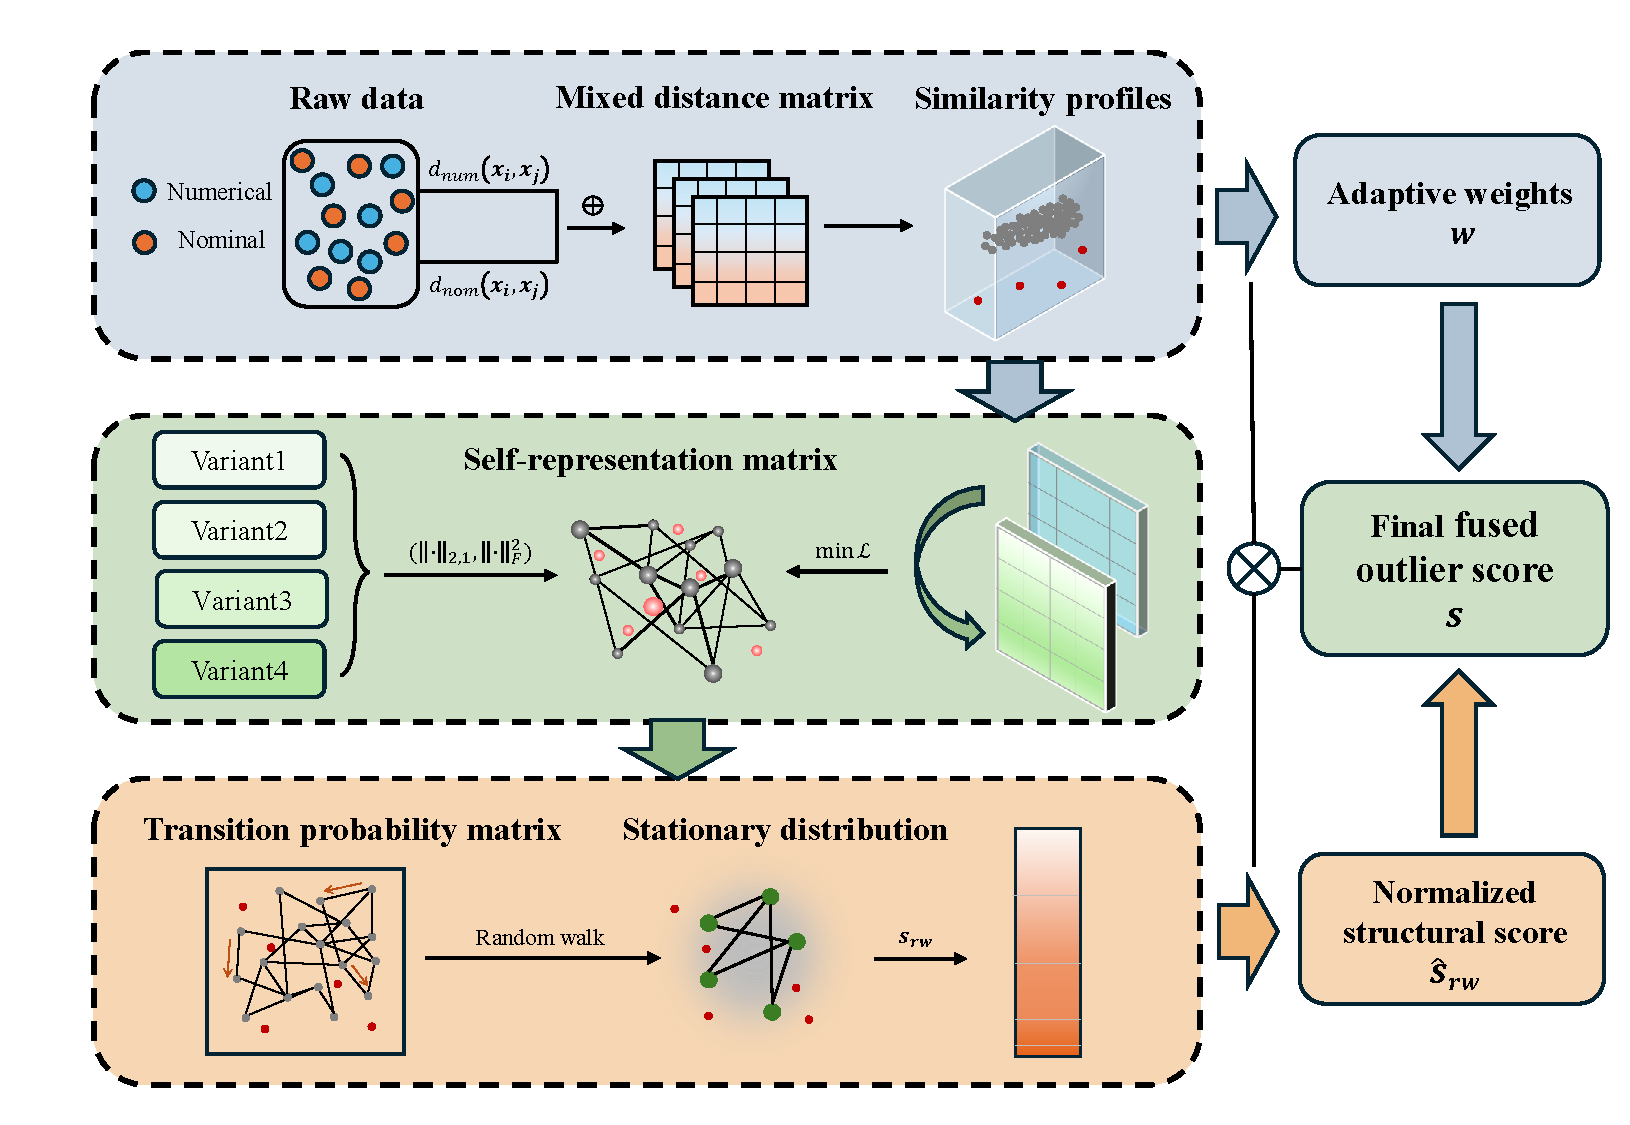
\includegraphics[width=\textwidth]{Figures/framework_KSRA.pdf} 
    \caption{The framework of KSRA.}
    \label{fig:KSRA_framework}
\end{figure*}


\begin{algorithm}
\caption{\enskip KSRA algorithm}\label{alg1}
\begin{algorithmic}
    \State \textbf{Input:} Data matrix $\boldsymbol{X} \in \mathbb{R}^{n \times m}$, regularization parameter $\lambda$, and a self-representation variant.
    \State \textbf{Output:} Final outlier score $\boldsymbol{s}$.

    \State Compute the hybrid distance matrix $\boldsymbol{D}$
    \State Set the Gaussian bandwidth $\sigma = \frac{1}{n(n-1)}\sum_{i\ne j}d_{ij}$ and the restart probability $d=0.85$
    
    \State Construct the similarity-profile matrix $\boldsymbol{K}$ by Eq.~(\ref{kernel_matrix})
    \State Compute the adaptive weights $w_{i}$ by Eq.~(\ref{initial_anomaly_belief})

    \State Solve the selected self-representation model using Eqs.~(\ref{Case1}), (\ref{Case2}), (\ref{Case3}) or (\ref{Case4}), as appropriate.
    
    \State Construct the transition matrix $\boldsymbol{P}$ by Eq.~(\ref{transition_probability})
    \State Compute the random walk steady-state score $\boldsymbol{s}_{rw}$ by Eq.~(\ref{randomwalk_outlier_score})
    \State Calculate the final fused outlier score $\boldsymbol{s}$ by Eq.~(\ref{fuse_outlier_score})
    
    \State \Return $\boldsymbol{s}$
\end{algorithmic}
\end{algorithm}

\section{Experiments}\label{Experiments}

In this section, we introduced the datasets and comparison algorithms employed, along with several experiments applied in our method. Analysis is conducted based on Receiver Operating
Characteristic (ROC) curves and Area Under the ROC
Curve (AUC) results, statistical hypothesis testing, and other aspects, with experimental findings visualized.

\subsection{Experiments Setup}

We select 20 public datasets spanning diverse domains and scales, encompassing numerical attribute data, nominal attribute data, and mixed attribute data. These datasets are accessible via the public website\footnote{\url{https://github.com/BELLoney/Outlier-detection}}. Basic information about the datasets is presented in Table \ref{KSRA-DS}. We used the prepared benchmark data files. For these prepared benchmark files, columns with a maximum value of at most $1 + 10^{-9}$ were assigned to the numerical group for Euclidean distance. The remaining columns contained integer-coded values and were assigned to the nominal group for normalized Hamming distance. Table \ref{KSRA-DS} classifies each dataset according to these feature groups. In the prepared inputs, missing entries correspond to column-modal values for partially observed columns, while entirely missing columns are represented by constants. No additional imputation was performed during the experiments.

Also, we evaluate the performance of our method on 20 datasets in comparison with 11 representative anomaly detection algorithms, including AutoEncoder \cite{hinton2006reducing}, Variational AutoEncoder (VAE) \cite{kingma2013auto}, Variance Structural Score (VarE) \cite{8526528}, Weighted Neighbourhood Information Network based Outlier Detection (WNINOD) \cite{wang2021outlier}, Empirical-Cumulative-Distribution-based Outlier Detection (ECOD) \cite{li2022ecod}, Rotation-based Outlier Detection (ROD) \cite{almardeny2020novel}, Incomplete Local and Global Neighborhood Information (ILGNI) network \cite{li2023incomplete}, Deep Isolation Forest (DIF) \cite{xu2023deep}, Fusing Multi-scale Fuzzy Information to Detect Outliers (MFIOD) \cite{chen2024fusing}, Granule Density-based Anomaly Detection (GDAD) \cite{chen2025integrating}, and the Granular-ball Mean-shift Outlier Detector (GBMOD) \cite{cheng2025gbmod}. 

For these comparison methods, we set reasonable parameter ranges based on relevant papers to ensure favorable detection performance. For example, the hyper-parameter adjustment ranges of VarE varies in $\{10^i \mid i \in \{-3, -2, \dots, 3\}\}$, WNINOD in $[1,10]$, while GBMOD using $k \in[2,60]$ with a stepsize of 1. For each dataset and KSRA variant, we selected $\lambda$ from $\{10^{-8}, 10^{-7},\cdots, 10^{7}\}$ by maximizing evaluation ROC-AUC among configurations that met the convergence criteria. The detector was fitted using unlabeled inputs, but $\lambda$ selection used the evaluation labels. Each iterative solve is limited to 20,000 iterations and a nominal time budget of 120 s, checked between iterations.

We employ the ROC curve and the AUC as the primary evaluation metrics \cite{campos2016evaluation}. The ROC curve illustrates the trade-off between the True Positive Rate (TPR) and the False Positive Rate (FPR) across various decision thresholds. The AUC value, representing the area under the ROC curve, provides a scalar measure of the overall classification performance. An AUC value closer to 1 indicates a superior capability of the algorithm to correctly rank anomalous instances higher than normal ones. Stochastic baselines were evaluated using single runs; their reported results do not quantify variability across random seeds.


\begin{table*}[!ht]
	\caption{Basic information of experimental datasets.}\label{KSRA-DS}
    \centering
	% \resizebox{1\textwidth}{!}{
		\begin{tabular}{lllccccc}
			\toprule
			ID & Datasets & Abbr. & Type & Attributes & Objects & Outliers & Outlier ratios \\\midrule
            1 & Annealing\_variant1 & Annealing & Mixed & 38 & 798 & 42 & 5.26\% \\
            2 & Arrhythmia\_variant1 & Arrhythmia & Mixed & 279 & 452 & 66 & 14.60\% \\
            3 & Audiology\_variant1 & Audio & Nominal & 69 & 226 & 57 & 25.22\% \\
            4 & Bands\_band\_6\_variant1 & Bands & Mixed & 39 & 318 & 6 & 1.89\% \\
            5 & Cardio & Cardio & Numerical & 21 & 1831 & 176 & 9.61\% \\
            6 & Cardiotocography\_2and3\_33\_variant1 & Cardio\_33 & Numerical & 21 & 1688 & 33 & 1.95\% \\
            7 & Chess\_nowin\_16\_variant1 & Chess\_16 & Mixed & 36 & 1685 & 16 & 0.95\% \\
            8 & Chess\_nowin\_34\_variant1 & Chess\_34 & Mixed & 36 & 1703 & 34 & 2.00\% \\
            9 & Ecoli & Ecoli & Numerical & 7 & 336 & 9 & 2.68\% \\
            10 & Iris\_Irisvirginica\_11\_variant1 & Iris & Numerical & 4 & 111 & 11 & 9.91\% \\
            11 & Lymphography & Lymphography & Nominal & 18 & 148 & 6 & 4.05\% \\
            12 & Monks\_0\_4\_variant1 & Monks & Nominal & 6 & 232 & 4 & 1.72\% \\
            13 & Mushroom\_p\_221\_variant1 & Mushroom & Mixed & 22 & 4429 & 221 & 4.99\% \\
            14 & Sick\_sick\_72\_variant1 & Sick & Mixed & 29 & 3613 & 72 & 1.99\% \\
            15 & Tic\_tac\_toe\_negative\_12\_variant1 & Tic\_12 & Nominal & 9 & 638 & 12 & 1.88\% \\
            16 & Tic\_tac\_toe\_negative\_32\_variant1 & Tic\_32 & Nominal & 9 & 658 & 32 & 4.86\% \\
            17 & Vote\_republican\_29\_variant1 & Vote & Nominal & 16 & 296 & 29 & 9.80\% \\
            18 & Wbc\_malignant\_39\_variant1 & Wbc & Numerical & 9 & 483 & 39 & 8.07\% \\
            19 & Wdbc\_M\_39\_variant1 & Wdbc\_M & Numerical & 31 & 396 & 39 & 9.85\% \\
            20 & Yeast\_ERL\_5\_variant1 & Yeast & Numerical & 8 & 1141 & 5 & 0.44\% \\
            \bottomrule
        \end{tabular}
        \par\vspace{2pt}
        \parbox{\textwidth}{\footnotesize\textit{Note:} Type refers to the feature groups used for distance computation in KSRA, including retained constant columns.}
        % }
\end{table*}


\subsection{Experimental Results}

Fig.\ref{fig:all_rocs} shows the ROC curves for the 20 benchmark datasets, with KSRA$_2$ highlighted in red. A curve closer to the upper-left corner indicates a better trade-off between the true-positive and false-positive rates. KSRA$_2$ achieves higher AUC than each of the 11 baselines on Annealing, Audio, Ecoli, and Tic\_32, with the largest margin among these four datasets on Audio. It also leads the baselines on Arrhythmia and matches the best baseline on Monks.

Table \ref{tab:KSRA-AUC} reports the ROC-AUC values for the 11 baselines and the four KSRA variants described in Section 5.4. The highest and second-highest distinct displayed values are shown in bold and underlined, respectively. KSRA$_2$ is the fixed variant used for the main comparison across datasets. KSRA$_{best}$ selects the highest AUC across the four variants on each dataset. It is included in the table as an oracle reference and excluded from fixed-method rankings and statistical tests. The results support the following observations.

\begin{enumerate}[\indent (1)]
    \item Across the 20 datasets, KSRA$_2$ achieves a mean AUC of 0.946, compared with 0.923 for GBMOD, the baseline with the highest mean AUC. Using ROC-AUC values rounded to nine decimal places, KSRA$_2$ exceeds the best of the 11 original baselines on nine datasets, ties it on four, and trails it on seven. The deficits on Cardio and Cardio\_33 are approximately 0.014 and 0.013, respectively, while the deficit on Mushroom is below 0.009.
    \item Among the four variants, KSRA$_2$ achieves the highest mean AUC (0.946), followed by KSRA$_3$ (0.941) and KSRA$_1$ (0.936). KSRA$_2$ also has the shortest mean runtime among the four variants, at 1.669 s for the selected configurations. The mean AUC of the oracle reference is 0.947, only 0.0009 higher than that of KSRA$_2$. KSRA$_4$ yields a lower mean AUC of 0.775 under the current budget, with all 16 parameter settings converging on four datasets. Its reported AUC therefore reflects the best performance among the settings that converged.
    \item The performance deficits on Sick and Wdbc\_M differ substantially. On Sick, KSRA$_2$ achieves an AUC of 0.811, compared with 0.895 for ROD. On Wdbc\_M, the difference from VarE, the strongest baseline, is approximately 0.0004. These results show that the margin varies across datasets, even though KSRA$_2$ achieves the highest mean AUC under the reported evaluation protocol.
\end{enumerate}

To complement the original comparison in Table \ref{tab:KSRA-AUC}, we evaluate the four KSRA variants against a recent deep graph anomaly detector, DVGAE-GAN \cite{khan2024anomalous}, together with established kernel-based methods, Kernel PCA \cite{hoffmann2007kernel} and OCSVM-RBF \cite{scholkopf2001estimating}, and the low-rank self-representation method LRR \cite{liu2012exact}. All methods are evaluated on the same 20 benchmark datasets. Since the benchmark datasets do not provide observed network edges, we adapt DVGAE-GAN by constructing symmetric kNN graphs with RBF edge weights from the preprocessed attributes. We use $k=10$, a latent dimension of 32, and 200 training epochs. The reported results correspond to this adapted implementation on the tabular benchmarks. The four variants employ different combinations of reconstruction losses and regularization terms, and their results are reported separately in Table \ref{tab:additional_baselines} to examine the performance of the different formulations. Additionally, KSRA$_{best}$ denotes the highest AUC among the four variants on each dataset. It serves only as an oracle best-variant reference, rather than an independently specified method.

\begin{enumerate}[\indent (1)]
    \item KSRA$_2$ achieves the highest mean AUC among the four fixed variants (0.9460), followed by KSRA$_3$ (0.9409). Their mean AUCs exceed that of OCSVM-RBF, the strongest additional baseline on average (0.9386), by 0.74 and 0.23 percentage points, respectively.

    \item KSRA$_1$ achieves a mean AUC of 0.9360, exceeding DVGAE-GAN, Kernel PCA, and LRR while trailing OCSVM-RBF. KSRA$_4$ achieves a mean AUC of 0.7747 under the current solver budget, below all four additional baselines.

    \item Using the same nine-decimal comparison, KSRA$_2$ exceeds the best of the four additional baselines on seven datasets, ties it on four, and trails it on nine. Its largest gains are on Annealing and Arrhythmia, where its AUC exceeds that of the strongest additional baseline by 0.060 and 0.039, respectively.

    \item The additional baselines remain competitive on several datasets. Kernel PCA outperforms all four KSRA variants on Bands, Chess\_16, Chess\_34, and Mushroom, and achieves an AUC of 1.000 on both Tic\_12 and Tic\_32. LRR leads all four variants on Cardio, while OCSVM-RBF leads them on Cardio\_33 and Sick.
\end{enumerate}



\begin{figure*}[t!]
    \centering
    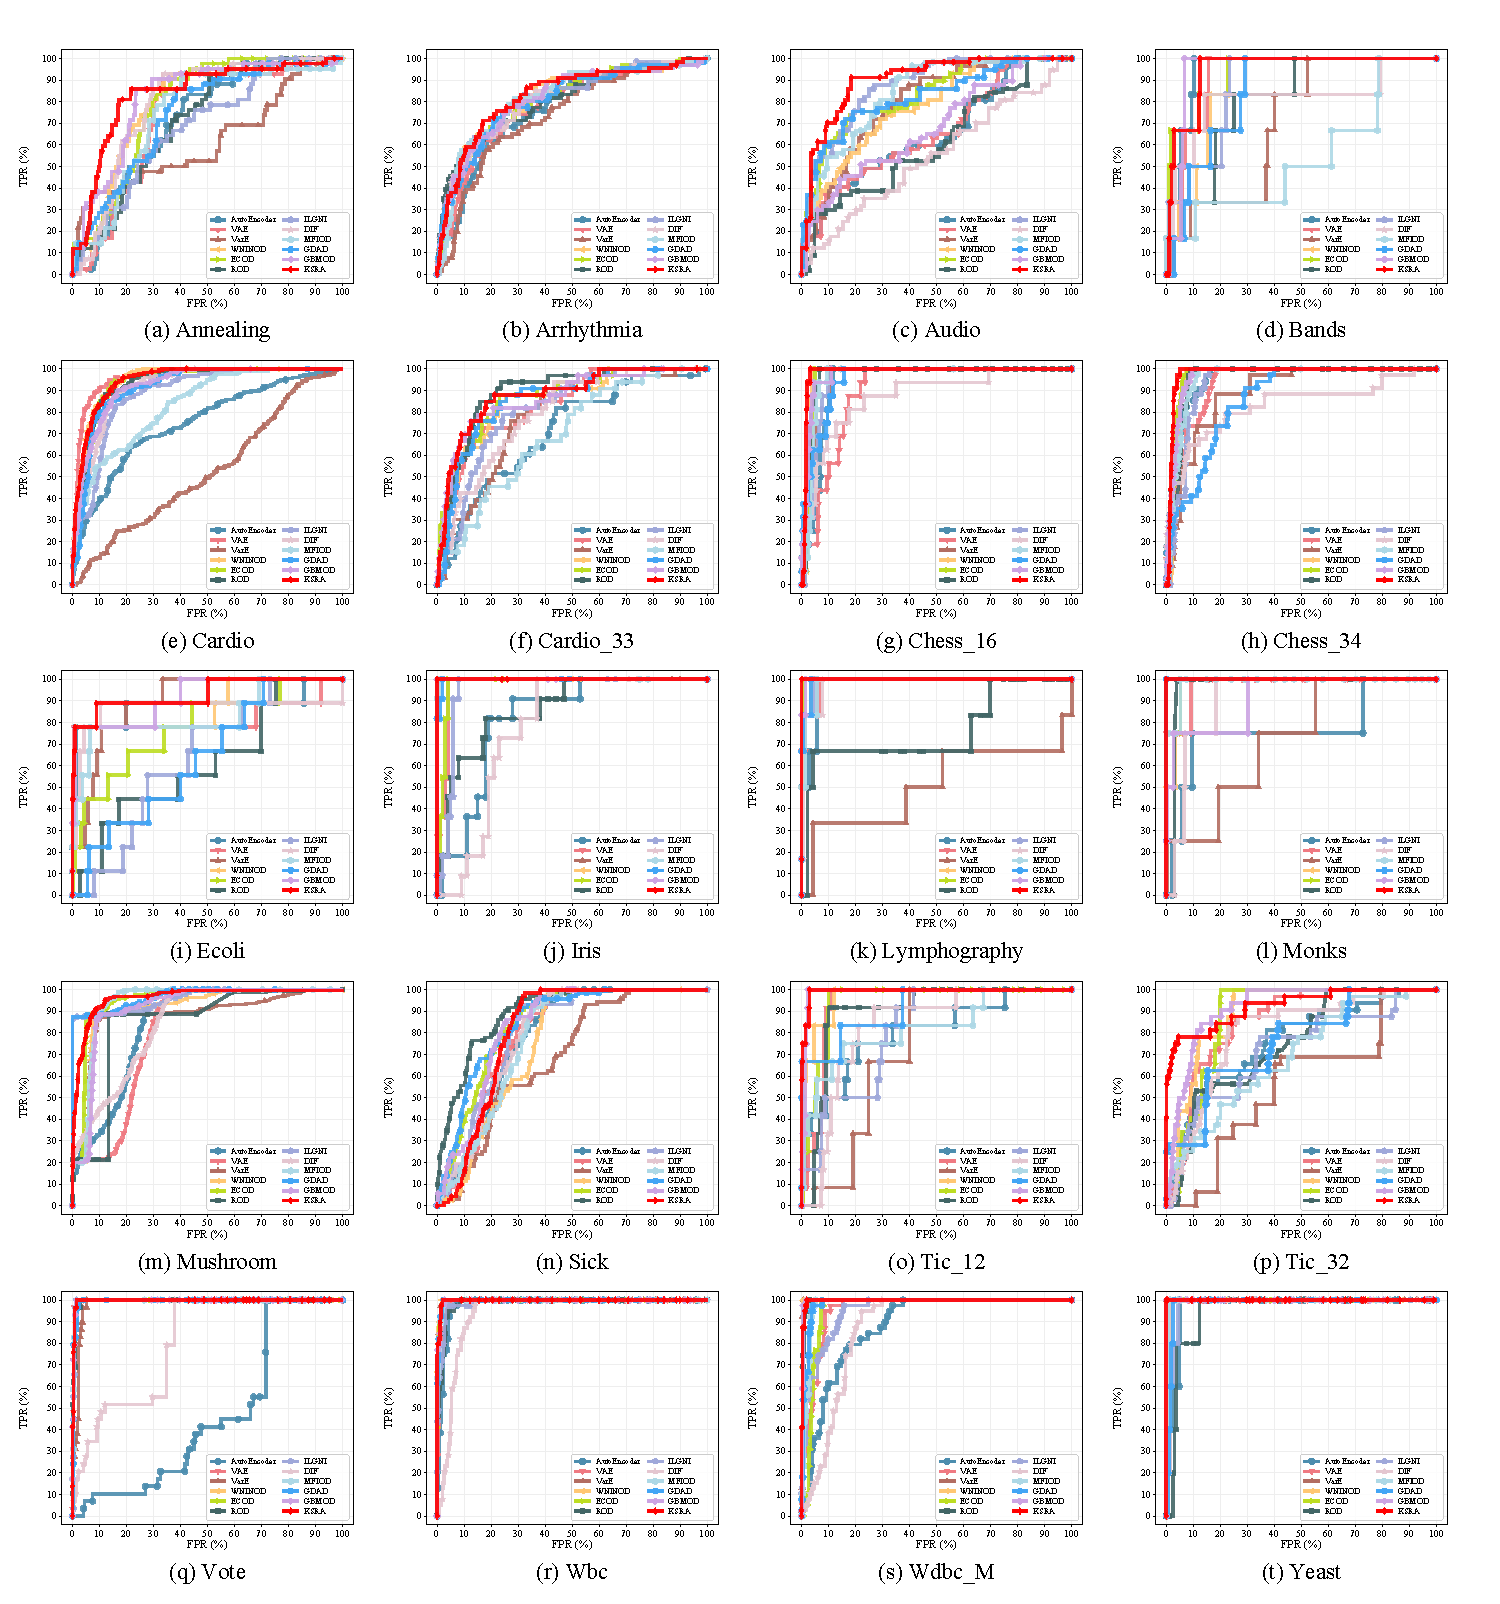
\includegraphics[width=\textwidth]{Figures/Fig2_ROC.pdf}
    \caption{ROC curves on 20 datasets. The red curve denotes KSRA$_2$ with the selected $\lambda$.}
    \label{fig:all_rocs}
\end{figure*}



% Requires booktabs and graphicx.
\begin{table*}[!ht]
    \centering
    \caption{ROC-AUC on 20 benchmark datasets.}
    \label{tab:KSRA-AUC}
    \resizebox{\textwidth}{!}{%
        \begin{tabular}{lccccccccccc|cccc|c}
            \toprule
            Datasets & AutoEncoder & VAE & VarE & WNINOD & ECOD & ROD & ILGNI & DIF & MFIOD & GDAD & GBMOD & KSRA$_1$ & KSRA$_2$ & KSRA$_3$ & KSRA$_4$ & KSRA$_{best}$ \\
            \midrule
            Annealing & 0.714 & 0.741 & 0.619 & 0.791 & 0.787 & 0.712 & 0.686 & 0.792 & 0.743 & 0.741 & 0.822 & 0.834 & \underline{0.836} & \textbf{0.842} & 0.500 & \textbf{0.842} \\
            Arrhythmia & 0.768 & 0.780 & 0.739 & 0.815 & 0.807 & 0.801 & 0.816 & 0.809 & 0.816 & 0.806 & 0.810 & 0.823 & \underline{0.826} & \textbf{0.827} & \underline{0.826} & \textbf{0.827} \\
            Audio & 0.655 & 0.666 & 0.792 & 0.778 & 0.833 & 0.615 & 0.873 & 0.549 & 0.842 & 0.825 & 0.681 & 0.898 & \textbf{0.904} & \underline{0.902} & 0.898 & \textbf{0.904} \\
            Bands & 0.939 & 0.917 & 0.702 & 0.882 & 0.936 & 0.808 & 0.874 & 0.816 & 0.545 & 0.848 & 0.948 & \underline{0.949} & 0.947 & \textbf{0.950} & \textbf{0.950} & \textbf{0.950} \\
            Cardio & 0.751 & \textbf{0.962} & 0.526 & \underline{0.949} & 0.935 & 0.932 & 0.887 & 0.918 & 0.834 & 0.918 & 0.925 & 0.946 & 0.948 & 0.946 & 0.500 & 0.948 \\
            Cardio\_33 & 0.711 & 0.838 & 0.780 & 0.851 & 0.871 & \textbf{0.893} & 0.811 & 0.796 & 0.697 & 0.858 & 0.864 & 0.877 & \underline{0.880} & \underline{0.880} & 0.500 & \underline{0.880} \\
            Chess\_16 & 0.939 & 0.894 & 0.956 & \underline{0.975} & 0.969 & 0.972 & 0.950 & 0.877 & 0.961 & 0.951 & 0.973 & 0.972 & \textbf{0.984} & 0.972 & 0.500 & \textbf{0.984} \\
            Chess\_34 & 0.959 & 0.936 & 0.892 & 0.964 & 0.968 & 0.954 & 0.935 & 0.830 & 0.957 & 0.863 & \underline{0.969} & 0.961 & \textbf{0.980} & 0.961 & 0.500 & \textbf{0.980} \\
            Ecoli & 0.877 & 0.820 & 0.899 & 0.874 & 0.781 & 0.613 & 0.638 & 0.864 & 0.835 & 0.635 & \underline{0.918} & 0.900 & \textbf{0.932} & 0.900 & 0.913 & \textbf{0.932} \\
            Iris & 0.823 & 0.975 & \textbf{1.000} & \textbf{1.000} & 0.977 & 0.866 & 0.951 & 0.779 & \underline{0.999} & 0.997 & \textbf{1.000} & \underline{0.999} & \textbf{1.000} & \underline{0.999} & \underline{0.999} & \textbf{1.000} \\
            Lymphography & 0.977 & 0.987 & 0.507 & 0.992 & 0.996 & 0.762 & 0.991 & 0.982 & 0.986 & 0.993 & \underline{0.998} & 0.989 & \textbf{1.000} & \underline{0.998} & 0.993 & \textbf{1.000} \\
            Monks & 0.774 & 0.977 & 0.727 & 0.978 & \underline{0.987} & 0.968 & \textbf{1.000} & 0.912 & \underline{0.987} & \textbf{1.000} & 0.917 & \textbf{1.000} & \textbf{1.000} & \textbf{1.000} & \textbf{1.000} & \textbf{1.000} \\
            Mushroom & 0.849 & 0.805 & 0.880 & 0.912 & 0.949 & 0.847 & 0.961 & 0.847 & 0.940 & \textbf{0.970} & 0.916 & 0.953 & \underline{0.962} & 0.953 & 0.500 & \underline{0.962} \\
            Sick & 0.784 & 0.798 & 0.691 & 0.754 & 0.843 & \textbf{0.895} & 0.807 & 0.797 & 0.778 & \underline{0.851} & 0.833 & 0.790 & 0.811 & 0.804 & 0.500 & 0.811 \\
            Tic\_12 & 0.803 & 0.936 & 0.733 & 0.967 & 0.948 & 0.900 & 0.813 & 0.829 & 0.824 & 0.913 & 0.989 & 0.984 & \underline{0.994} & \textbf{0.995} & \textbf{0.995} & \textbf{0.995} \\
            Tic\_32 & 0.763 & 0.854 & 0.563 & 0.894 & 0.878 & 0.749 & 0.722 & 0.801 & 0.695 & 0.758 & 0.917 & 0.857 & \underline{0.926} & 0.897 & \textbf{0.931} & \textbf{0.931} \\
            Vote & 0.464 & 0.995 & 0.981 & 0.995 & 0.995 & 0.995 & 0.994 & 0.801 & \underline{0.996} & 0.994 & \textbf{0.997} & \textbf{0.997} & \textbf{0.997} & \textbf{0.997} & \textbf{0.997} & \textbf{0.997} \\
            Wbc & 0.980 & 0.989 & \textbf{0.997} & \textbf{0.997} & \underline{0.995} & 0.985 & 0.988 & 0.939 & \underline{0.995} & \underline{0.995} & \textbf{0.997} & \textbf{0.997} & \textbf{0.997} & \textbf{0.997} & \textbf{0.997} & \textbf{0.997} \\
            Wdbc\_M & 0.881 & 0.958 & \textbf{0.997} & \underline{0.996} & 0.959 & 0.995 & 0.951 & 0.871 & 0.981 & 0.985 & \underline{0.996} & 0.995 & \textbf{0.997} & \textbf{0.997} & \underline{0.996} & \textbf{0.997} \\
            Yeast & 0.971 & 0.994 & \textbf{1.000} & \underline{0.998} & 0.995 & 0.949 & 0.981 & 0.987 & 0.996 & 0.984 & \textbf{1.000} & \textbf{1.000} & \textbf{1.000} & \textbf{1.000} & 0.500 & \textbf{1.000} \\
            \midrule
            Average AUC & 0.819 & 0.891 & 0.799 & 0.918 & 0.921 & 0.861 & 0.881 & 0.840 & 0.870 & 0.894 & 0.923 & 0.936 & \textbf{0.946} & \underline{0.941} & 0.775 & 0.947 \\
            Average Runtime(s) & 2.137 & 5.811 & 3.408 & 35.353 & 0.057 & 1527.336 & 184.858 & 1.741 & 0.785 & 0.790 & 2.435 & 17.944 & 1.669 & 24.422 & 26.446 & - \\
            \bottomrule
        \end{tabular}%
    }
    \par\vspace{2pt}
    \parbox{\textwidth}{\footnotesize\textit{Note:} For each KSRA variant, the best result among converged configurations is reported. KSRA$_{best}$ is an oracle reference across variants. Bold and underlining mark the highest and second-highest distinct displayed values, including ties. Runtime values are descriptive; complete original environment metadata and repeated-run timing statistics were not retained.}
\end{table*}

% Requires booktabs and graphicx.
\begin{table*}[!ht]
    \centering
    \caption{AUC comparison of KSRA with additional baseline methods.}
    \label{tab:additional_baselines}
    \resizebox{0.8\textwidth}{!}{%
        \begin{tabular}{lcccc|cccc|c}
            \toprule
            Datasets & DVGAE-GAN & Kernel PCA & LRR & OCSVM-RBF & KSRA$_1$ & KSRA$_2$ & KSRA$_3$ & KSRA$_4$ & KSRA$_{best}$ \\
            \midrule
            Annealing & 0.754 & 0.776 & 0.751 & 0.743 & 0.834 & \underline{0.836} & \textbf{0.842} & 0.500 & \textbf{0.842} \\
            Arrhythmia & 0.785 & 0.782 & 0.787 & 0.758 & 0.823 & \underline{0.826} & \textbf{0.827} & \underline{0.826} & \textbf{0.827} \\
            Audio & 0.868 & 0.828 & 0.900 & 0.809 & 0.898 & \textbf{0.904} & \underline{0.902} & 0.898 & \textbf{0.904} \\
            Bands & 0.882 & \textbf{0.952} & 0.887 & \textbf{0.952} & 0.949 & 0.947 & \underline{0.950} & \underline{0.950} & \underline{0.950} \\
            Cardio & 0.892 & 0.941 & \textbf{0.949} & 0.912 & 0.946 & \underline{0.948} & 0.946 & 0.500 & \underline{0.948} \\
            Cardio\_33 & 0.839 & 0.856 & 0.845 & \textbf{0.889} & 0.877 & \underline{0.880} & \underline{0.880} & 0.500 & \underline{0.880} \\
            Chess\_16 & 0.970 & \textbf{0.996} & 0.971 & \underline{0.990} & 0.972 & 0.984 & 0.972 & 0.500 & 0.984 \\
            Chess\_34 & 0.969 & \textbf{0.992} & 0.959 & \underline{0.984} & 0.961 & 0.980 & 0.961 & 0.500 & 0.980 \\
            Ecoli & 0.856 & 0.889 & 0.897 & \underline{0.931} & 0.900 & \textbf{0.932} & 0.900 & 0.913 & \textbf{0.932} \\
            Iris & 0.850 & 0.959 & 0.627 & \textbf{1.000} & \underline{0.999} & \textbf{1.000} & \underline{0.999} & \underline{0.999} & \textbf{1.000} \\
            Lymphography & 0.991 & \textbf{1.000} & \underline{0.998} & \textbf{1.000} & 0.989 & \textbf{1.000} & \underline{0.998} & 0.993 & \textbf{1.000} \\
            Monks & 0.764 & \textbf{1.000} & \underline{0.987} & \textbf{1.000} & \textbf{1.000} & \textbf{1.000} & \textbf{1.000} & \textbf{1.000} & \textbf{1.000} \\
            Mushroom & 0.973 & \textbf{0.979} & \underline{0.975} & \textbf{0.979} & 0.953 & 0.962 & 0.953 & 0.500 & 0.962 \\
            Sick & 0.794 & \underline{0.835} & 0.770 & \textbf{0.847} & 0.790 & 0.811 & 0.804 & 0.500 & 0.811 \\
            Tic\_12 & 0.855 & \textbf{1.000} & \textbf{1.000} & \textbf{1.000} & 0.984 & 0.994 & \underline{0.995} & \underline{0.995} & \underline{0.995} \\
            Tic\_32 & 0.770 & \textbf{1.000} & \textbf{1.000} & \textbf{1.000} & 0.857 & 0.926 & 0.897 & \underline{0.931} & \underline{0.931} \\
            Vote & 0.325 & 0.650 & \underline{0.995} & 0.994 & \textbf{0.997} & \textbf{0.997} & \textbf{0.997} & \textbf{0.997} & \textbf{0.997} \\
            Wbc & 0.972 & 0.990 & 0.814 & \underline{0.996} & \textbf{0.997} & \textbf{0.997} & \textbf{0.997} & \textbf{0.997} & \textbf{0.997} \\
            Wdbc\_M & 0.805 & 0.971 & 0.883 & 0.989 & 0.995 & \textbf{0.997} & \textbf{0.997} & \underline{0.996} & \textbf{0.997} \\
            Yeast & 0.996 & \underline{0.999} & 0.995 & \textbf{1.000} & \textbf{1.000} & \textbf{1.000} & \textbf{1.000} & 0.500 & \textbf{1.000} \\
            \midrule
            Average AUC & 0.845 & 0.920 & 0.900 & 0.939 & 0.936 & \textbf{0.946} & \underline{0.941} & 0.775 & 0.947 \\
            \bottomrule
        \end{tabular}%
    }
\end{table*}



\subsection{Evaluation Using Average Precision}

To complement ROC-AUC, particularly on datasets with low anomaly prevalence, we report average precision (AP) across the 20 benchmark datasets. Treating anomalies as the positive class, we compute non-interpolated AP as
\begin{equation*}\label{AP_equ}
    \mathrm{AP}=\sum_{k=1}^{K}(R_k-R_{k-1})P_k,
\end{equation*}
where $P_k$ and $R_k$ denote precision and recall at the $k$-th score threshold, respectively, and $R_0=0$. Higher AP indicates a better balance between retrieving anomalies and limiting false positives. 

AP is computed from per-sample anomaly scores using the configurations selected for the ROC-AUC evaluation, without further tuning for AP. Table \ref{tab:ap_comparison} reports the results for 15 baselines and four KSRA variants, with an unweighted mean across datasets. KSRA$_{best}$ reports the AP of the variant with the highest ROC-AUC on each dataset, with exact ties resolved by choosing the variant with the smaller index. This oracle reference is included in the table. Bold and underlining denote the highest and second-highest distinct displayed values, respectively, with ties retained.

\begin{enumerate}
    \item KSRA$_1$, KSRA$_2$, KSRA$_3$, and KSRA$_4$ achieve mean AP values of 0.6173, 0.6492, 0.6329, and 0.4829, respectively. KSRA$_2$ achieves the highest mean AP among the four fixed variants, consistent with their ordering at the top of the ROC-AUC comparison.

    \item OCSVM-RBF achieves the highest mean AP among the baselines (0.6637). KSRA$_2$ ranks second overall among the fixed methods, trailing OCSVM-RBF by 1.45 percentage points and exceeding the other 14 baselines in mean AP.
    
    \item The relative performance varies across datasets. KSRA$_2$ exceeds the strongest baseline in AP on Annealing, Audio, and Wdbc\_M, and ties the strongest baseline at 1.000 on Iris, Lymphography, Monks, and Yeast. On Chess\_16 and Chess\_34, KSRA$_2$ achieves ROC-AUC values of 0.984 and 0.980 but AP values of 0.226 and 0.320, respectively. Kernel PCA achieves AP values of 0.554 and 0.620 on these datasets. The contrast illustrates why AP complements ROC-AUC when anomalies are rare.
\end{enumerate}

% Requires booktabs and graphicx.
\begin{table*}[!ht]
    \centering
    \caption{Average precision comparison across 20 benchmark datasets.}
    \label{tab:ap_comparison}
    \resizebox{\textwidth}{!}{%
        \begin{tabular}{lccccccccccccccc|cccc|c}
            \toprule
            Datasets & AutoEncoder & VAE & VarE & WNINOD & ECOD & ROD & ILGNI & DIF & MFIOD & GDAD & GBMOD & DVGAE-GAN & Kernel PCA & LRR & OCSVM-RBF & KSRA$_1$ & KSRA$_2$ & KSRA$_3$ & KSRA$_4$ & KSRA$_{best}$ \\
            \midrule
            Annealing & 0.095 & 0.100 & 0.147 & 0.226 & 0.203 & 0.112 & 0.093 & 0.120 & 0.156 & 0.129 & 0.267 & 0.123 & 0.165 & 0.115 & 0.127 & \textbf{0.286} & \underline{0.278} & 0.270 & 0.053 & 0.270 \\
            Arrhythmia & 0.356 & 0.399 & 0.288 & 0.488 & 0.465 & \textbf{0.514} & \underline{0.494} & 0.457 & 0.404 & 0.480 & 0.468 & 0.448 & 0.430 & 0.454 & 0.421 & 0.470 & 0.476 & 0.476 & 0.475 & 0.476 \\
            Audio & 0.474 & 0.490 & 0.516 & 0.546 & 0.654 & 0.371 & 0.691 & 0.311 & 0.650 & 0.681 & 0.459 & 0.666 & 0.689 & 0.736 & 0.604 & 0.735 & \textbf{0.746} & \underline{0.742} & 0.735 & \textbf{0.746} \\
            Bands & 0.155 & 0.128 & 0.050 & 0.158 & \underline{0.423} & 0.107 & 0.284 & 0.153 & 0.190 & 0.080 & 0.182 & 0.136 & 0.321 & 0.266 & \textbf{0.425} & 0.247 & 0.246 & 0.241 & 0.249 & 0.241 \\
            Cardio & 0.304 & \textbf{0.701} & 0.105 & 0.645 & 0.567 & 0.554 & 0.439 & 0.551 & 0.424 & 0.494 & 0.577 & 0.516 & 0.632 & \underline{0.692} & 0.566 & 0.646 & 0.650 & 0.646 & 0.096 & 0.650 \\
            Cardio\_33 & 0.047 & 0.113 & 0.057 & 0.109 & 0.153 & 0.122 & 0.062 & 0.081 & 0.049 & 0.090 & \underline{0.154} & 0.128 & 0.118 & 0.094 & \textbf{0.156} & 0.137 & 0.139 & 0.140 & 0.020 & 0.140 \\
            Chess\_16 & 0.106 & 0.056 & 0.116 & 0.155 & 0.128 & 0.147 & 0.090 & 0.210 & 0.111 & 0.176 & 0.217 & 0.140 & \textbf{0.554} & 0.140 & \underline{0.360} & 0.144 & 0.226 & 0.144 & 0.009 & 0.226 \\
            Chess\_34 & 0.335 & 0.252 & 0.109 & 0.211 & 0.234 & 0.178 & 0.137 & 0.331 & 0.206 & 0.137 & 0.291 & 0.270 & \textbf{0.620} & 0.188 & \underline{0.443} & 0.194 & 0.320 & 0.194 & 0.020 & 0.320 \\
            Ecoli & 0.576 & 0.651 & 0.336 & 0.626 & 0.187 & 0.052 & 0.041 & 0.471 & 0.450 & 0.048 & 0.644 & 0.359 & 0.316 & \textbf{0.763} & 0.636 & 0.656 & \underline{0.728} & 0.656 & 0.658 & \underline{0.728} \\
            Iris & 0.287 & 0.776 & \textbf{1.000} & \textbf{1.000} & 0.713 & 0.429 & 0.531 & 0.200 & \underline{0.992} & 0.978 & \textbf{1.000} & 0.611 & 0.575 & 0.131 & \textbf{1.000} & \underline{0.992} & \textbf{1.000} & \underline{0.992} & \underline{0.992} & \textbf{1.000} \\
            Lymphography & 0.719 & 0.852 & 0.095 & 0.863 & 0.915 & 0.277 & 0.882 & 0.734 & 0.802 & 0.896 & \underline{0.958} & 0.859 & \textbf{1.000} & \underline{0.958} & \textbf{1.000} & 0.863 & \textbf{1.000} & \underline{0.958} & 0.842 & \textbf{1.000} \\
            Monks & 0.111 & 0.790 & 0.153 & 0.631 & \underline{0.812} & 0.239 & \textbf{1.000} & 0.122 & \underline{0.812} & \textbf{1.000} & 0.514 & 0.225 & \textbf{1.000} & \underline{0.812} & \textbf{1.000} & \textbf{1.000} & \textbf{1.000} & \textbf{1.000} & \textbf{1.000} & \textbf{1.000} \\
            Mushroom & 0.287 & 0.289 & 0.401 & 0.414 & 0.486 & 0.382 & 0.888 & 0.366 & 0.426 & 0.899 & 0.401 & \underline{0.900} & 0.891 & \textbf{0.901} & 0.681 & 0.885 & 0.663 & 0.885 & 0.050 & 0.663 \\
            Sick & 0.061 & 0.062 & 0.032 & 0.038 & 0.066 & \textbf{0.180} & 0.055 & 0.062 & 0.046 & 0.078 & 0.071 & 0.064 & 0.070 & 0.050 & \underline{0.088} & 0.042 & 0.047 & 0.045 & 0.020 & 0.047 \\
            Tic\_12 & 0.201 & 0.210 & 0.036 & 0.348 & 0.210 & 0.107 & 0.162 & 0.061 & 0.236 & 0.671 & 0.503 & 0.185 & \textbf{1.000} & \textbf{1.000} & \textbf{1.000} & 0.688 & 0.836 & 0.816 & \underline{0.852} & \underline{0.852} \\
            Tic\_32 & 0.154 & 0.164 & 0.056 & 0.209 & 0.171 & 0.118 & 0.120 & 0.133 & 0.158 & 0.345 & 0.284 & 0.168 & \textbf{1.000} & \textbf{1.000} & \textbf{1.000} & 0.585 & 0.728 & 0.607 & \underline{0.737} & \underline{0.737} \\
            Vote & 0.098 & 0.923 & 0.754 & 0.914 & 0.923 & 0.953 & 0.880 & 0.321 & 0.942 & 0.911 & \underline{0.965} & 0.070 & 0.140 & 0.930 & 0.947 & 0.960 & \underline{0.965} & 0.963 & \textbf{0.966} & \textbf{0.966} \\
            Wbc & 0.726 & 0.855 & \textbf{0.970} & 0.967 & 0.946 & 0.825 & 0.889 & 0.412 & 0.943 & 0.930 & 0.965 & 0.721 & 0.869 & 0.179 & 0.963 & 0.967 & \textbf{0.970} & \underline{0.968} & 0.967 & \textbf{0.970} \\
            Wdbc\_M & 0.387 & 0.623 & 0.951 & 0.920 & 0.543 & 0.894 & 0.675 & 0.298 & 0.755 & 0.832 & 0.915 & 0.344 & 0.685 & 0.432 & 0.857 & 0.906 & \underline{0.967} & \textbf{0.971} & 0.913 & \textbf{0.971} \\
            Yeast & 0.091 & 0.288 & \textbf{1.000} & 0.563 & 0.358 & 0.055 & 0.152 & 0.159 & 0.396 & 0.136 & \textbf{1.000} & 0.364 & 0.877 & 0.316 & \textbf{1.000} & \underline{0.943} & \textbf{1.000} & \underline{0.943} & 0.004 & \textbf{1.000} \\
            \midrule
            Average AP & 0.279 & 0.436 & 0.359 & 0.501 & 0.458 & 0.331 & 0.428 & 0.278 & 0.457 & 0.500 & 0.542 & 0.365 & 0.598 & 0.508 & \textbf{0.664} & 0.617 & \underline{0.649} & 0.633 & 0.483 & 0.650 \\
            \bottomrule
        \end{tabular}%
    }
\end{table*}



\subsection{Variant Analysis}\label{Variant Analysis}

The right part of Table \ref{tab:KSRA-AUC} presents the specific AUC values and average runtime experimental results for the variants. In particular, KSRA$_1$ represents the result obtained from Equation (\ref{Case1}) in the self-representation section; KSRA$_2$ denotes the results obtained from Eq.~(\ref{Case2}); KSRA$_3$ denotes the results obtained from Eq.~(\ref{Case3}), and KSRA$_4$ corresponds to Eq.~(\ref{Case4}). KSRA$_2$, which uses the squared Frobenius norm for both the reconstruction loss and coefficient regularization, achieves the highest mean ROC-AUC (0.9460) and the shortest mean runtime (1.669s) among the four variants. KSRA$_3$ achieves a similar mean ROC-AUC (0.9409), but its mean runtime is 24.422 s. All 16 regularization settings of KSRA$_2$ converged on each of the 20 datasets, whereas the other variants had incomplete convergence on some datasets. Their reported AUCs therefore reflect the best values among the configurations that converged within the prescribed budget.

KSRA$_2$ achieves the highest mean ROC-AUC among the four variants under the reported evaluation protocol. One possible explanation is that squared Frobenius regularization shrinks coefficients without explicitly promoting row sparsity, which may preserve weak but informative connections in the graph used for the random walk. The present comparison does not isolate the contribution of these connections, and incomplete convergence limits conclusions about the other variants. Computationally, KSRA$_2$ has a closed-form ridge solution and requires neither iterative reweighting nor ADMM. This difference in the solution procedure is consistent with its shorter measured runtime.


\subsection{Statistical Analysis}

Based on recent studies \cite{cheng2025gbmod,su2025identifying,su2025granular} on anomaly detection, we employed the non-parametric Friedman test supplemented by the Nemenyi post-hoc test to verify whether the performance improvement of our proposed KSRA method is statistically significant. This approach compares method ranks across datasets without assuming normally distributed AUC values. The Friedman test first confirms whether any overall differences exist among all methods, while the Nemenyi test further determines whether the performance gaps between algorithms significantly exceed the range of statistical random fluctuations. Throughout this analysis, KSRA denotes the fixed Frobenius norm variant, implemented as KSRA$_2$.

For the rank-based analysis, we rounded the ROC-AUC values to nine decimal places and assigned average ranks to ties within each dataset. The tie-corrected Friedman statistic was $\chi^2(11) = 91.86$, with an Iman-Davenport transformation of $F(11, 209) = 13.62$. The $F$ statistic exceeds the 0.05-level critical value of 1.835, indicating overall differences among the evaluated methods. We then used the Nemenyi post-hoc test for pairwise rank comparisons.

Fig.\ref{fig:CD_diagram} shows the average ranks and the critical difference of 3.7261 at $\alpha = 0.05$. The horizontal axis at the top of the figure represents the average rank of all evaluated methods across all datasets. Each method's position on the axes corresponds to its average rank. If two or more algorithms are connected by a horizontal red line segment, it indicates that the performance difference between them is not statistically significant. Conversely, if no line segment connects two algorithms, it signifies that they exhibit a statistically significant difference at the $\alpha = 0.05$ level.

\begin{enumerate}[\indent (1)]
    \item Our KSRA method achieves the best average rank (1.750) and ranks significantly better than AutoEncoder, VAE, VarE, ROD, ILGNI, DIF, MFIOD, and GDAD.
    \item GBMOD, WNINOD, and ECOD achieve average ranks of 3.600, 4.675, and 4.850, respectively. Their rank gaps from KSRA are 1.850, 2.925, and 3.100, all below the critical difference.
    \item The leading average rank summarizes KSRA's performance under the reported ROC-AUC selection and evaluation protocol. The pairwise results establish significant rank advantages over eight of the eleven baselines.
\end{enumerate}

To complement the overall rank-based comparisons, we additionally conduct two-sided Wilcoxon signed-rank tests between KSRA and each baseline, applying Holm correction across all 11 comparisons to control the family-wise error rate. Table \ref{tab:wilcoxon_holm} summarizes the mean and median AUC differences, win/tie/loss counts, and raw and adjusted $p-$values. AUC differences are calculated as the AUC of KSRA minus that of the corresponding baseline; positive values favor KSRA. Win/tie/loss counts describe numerical outcomes rather than dataset-level significance. To match the precision of the supplied baseline AUC, paired differences are rounded to nine decimal places for testing and counting. Zero differences are excluded, tied absolute differences receive average ranks, and two-sided $p-$values are calculated from the exact sign-permutation distribution.

\begin{enumerate}[\indent (1)]
    \item KSRA has positive mean and median ROC-AUC differences against all 11 baselines. The mean differences range from 0.022569 against GBMOD to 0.146959 against VarE. All 11 paired comparisons remain significant after Holm correction at $\alpha=0.05$.

    \item Against GBMOD, WNINOD, and ECOD, KSRA achieves win/tie/loss counts of 15/3/2, 18/1/1, and 19/0/1, respectively. The corresponding Holm-adjusted $p$-values are 0.002090, 0.000134, and 0.000839.
\end{enumerate}

The analyses address different comparisons: Nemenyi uses average-rank gaps across all method pairs, whereas Wilcoxon-Holm uses the signed ranks of paired AUC differences for the 11 comparisons with KSRA. These findings are conditional on the benchmark datasets and tuning protocol. Because some benchmark datasets are variants of the same source dataset, independence across benchmark tasks cannot be assumed.

\begin{figure*}
    \centering
    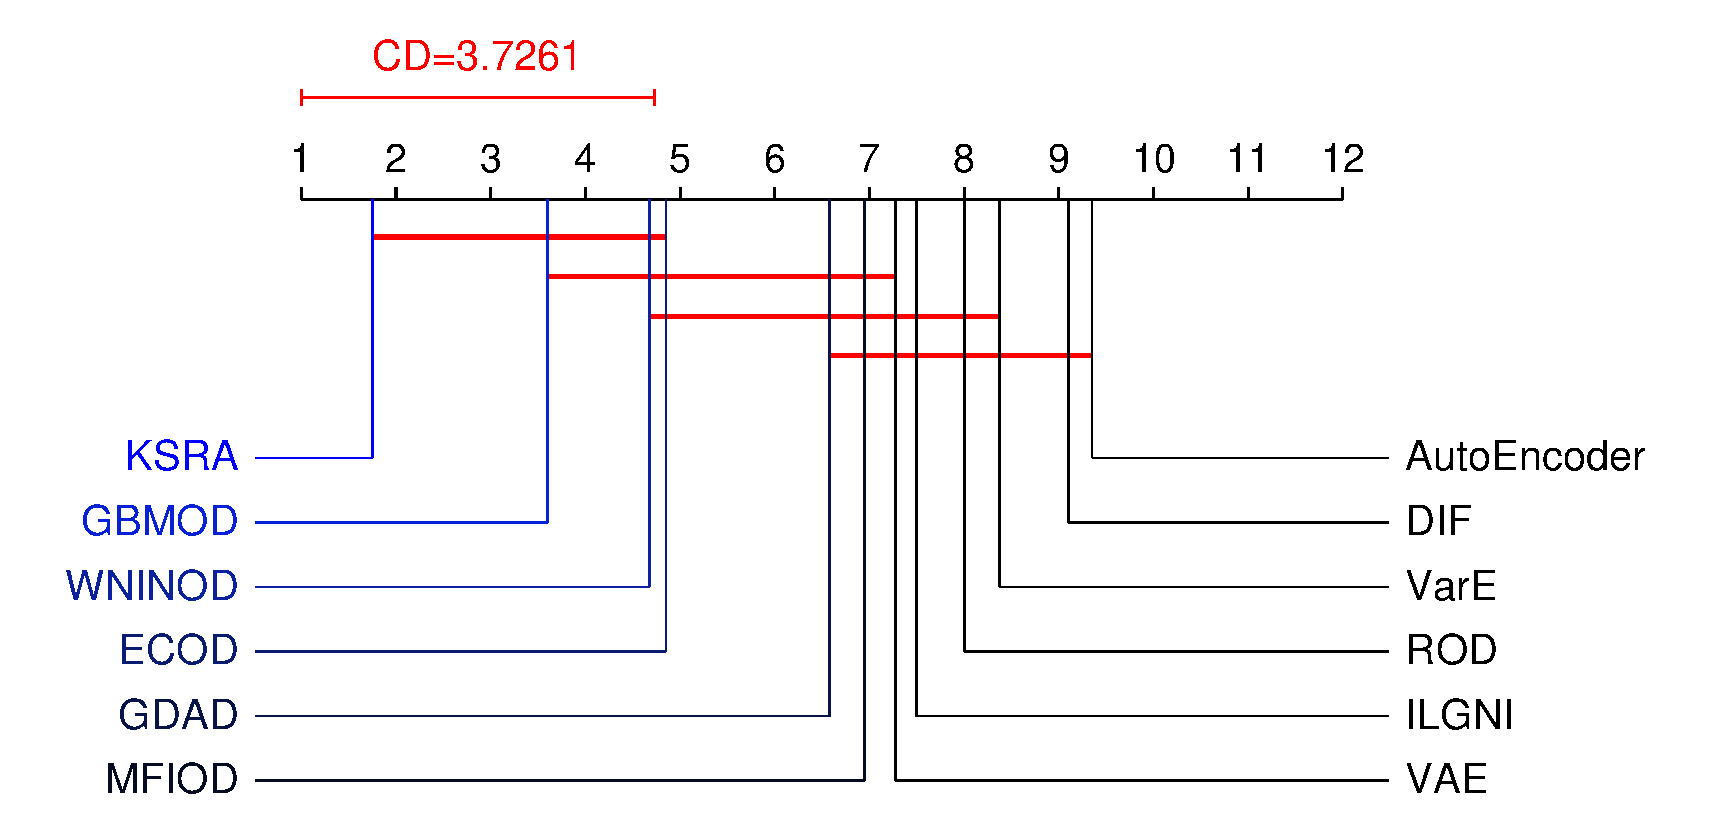
\includegraphics[scale=0.4]{Figures/CD_diagram.pdf}
    \caption{Nemenyi test figure on AUC.}
    \label{fig:CD_diagram}
\end{figure*}

\begin{table*}[!ht]
    \centering
    \caption{Pairwise ROC-AUC comparisons between KSRA and the 11 baselines using two-sided Wilcoxon signed-rank tests with Holm correction.}
    \label{tab:wilcoxon_holm}
    \resizebox{0.8\textwidth}{!}{
        \begin{tabular}{lrrrrrr}
            \hline
            Baseline & Mean $\Delta$AUC & Median $\Delta$AUC & W/T/L & $p$ & $p_{\mathrm{Holm}}$ & Sig. \\
            \hline
            AutoEncoder & +0.127080 & +0.114522 & 20/0/0 & 1.90735e-06 & 2.09808e-05 & Yes \\
            VAE & +0.054959 & +0.040462 & 19/0/1 & 2.67029e-05 & 0.000160217 & Yes \\
            VarE & +0.146959 & +0.093889 & 16/2/2 & 3.8147e-05 & 0.000190735 & Yes \\
            WNINOD & +0.027909 & +0.018745 & 18/1/1 & 1.90735e-05 & 0.000133514 & Yes \\
            ECOD & +0.025537 & +0.012991 & 19/0/1 & 0.000209808 & 0.000839233 & Yes \\
            ROD & +0.085527 & +0.041339 & 18/0/2 & 0.000322342 & 0.000967026 & Yes \\
            ILGNI & +0.064632 & +0.040047 & 19/1/0 & 3.8147e-06 & 3.05176e-05 & Yes \\
            DIF & +0.106200 & +0.097691 & 20/0/0 & 1.90735e-06 & 2.09808e-05 & Yes \\
            MFIOD & +0.075733 & +0.023486 & 20/0/0 & 1.90735e-06 & 2.09808e-05 & Yes \\
            GDAD & +0.051748 & +0.021047 & 17/1/2 & 0.000789642 & 0.00157928 & Yes \\
            GBMOD & +0.022569 & +0.009457 & 15/3/2 & 0.00209045 & 0.00209045 & Yes \\
            \hline
        \end{tabular}
    }
\end{table*}



\subsection{Hyper-parameter Sensitivity Analysis}

To examine hyperparameter sensitivity, we evaluate the fixed variant KSRA$_2$ on 20 benchmark datasets, varying one parameter at a time. We vary the regularization parameter $\lambda$ over $\{10^{-8},10^{-7},\ldots,10^7\}$ while fixing $\sigma=\sigma_0$ and $d=0.85$. We vary the restart weight $d$ over $\{0.05,0.10,0.15,0.30,0.50,0.70,0.85,0.95\}$ while fixing $\sigma=\sigma_0$. For the bandwidth sweep, we set $\sigma=\alpha\sigma_0$, with $\alpha\in\{0.25,0.5,0.75,1,1.25,1.5,2,4\}$, and fix $d=0.85$. Here, $\sigma_0$ is the mean off-diagonal mixed distance for each dataset. In both the restart-weight and bandwidth sweeps, we fix $\lambda$ to the value selected by ROC-AUC for that dataset at the default bandwidth and restart weight. Fig.\ref{fig:parameters_sensitivity} shows ten datasets per panel. The four Mushroom configurations at $\alpha\in\{1.25,1.5,2,4\}$ did not satisfy the convergence criterion, so their AUCs are omitted.

Across datasets, the median difference between the highest and lowest valid AUCs is 0.305 for $\lambda$, 0.150 for $\sigma/\sigma_0$, and 0.001 for $d$. The following observations summarize the responses over the tested grids.

\begin{enumerate}[\indent (1)]
    \item The response to $\lambda$ is nonmonotonic. On Chess\_34, the AUC decreases from 0.980 at $\lambda=10^{-5}$ to 0.089 at $\lambda=10$, then recovers to 0.962 at $\lambda=10^5$. Across the 20 datasets, the mean AUC ranges from 0.9257 to 0.9269 for the three tested values from $10^5$ to $10^7$. Smaller values remain preferable on some datasets. For example, Ecoli achieves an AUC of 0.932 at $\lambda=10^{-8}$ and 0.904 at each of the three largest tested values.

    \item The mean AUC changes from 0.9449 at $d=0.05$ to 0.9461 at $d=0.95$. The largest within-dataset AUC range over the tested restart weights is approximately 0.0137. These results indicate limited sensitivity to $d$ at the fixed bandwidth and the selected $\lambda$ for each dataset.

    \item The response to bandwidth varies across datasets. Iris achieves an AUC of 1.000 at $\alpha=1$, drops to 0.069 at $\alpha=2$, and recovers to 0.817 at $\alpha=4$. On Sick, the AUC decreases from 0.870 at $\alpha=0.25$ to 0.798 at $\alpha=4$. The best tested bandwidth multiplier therefore varies across datasets.
\end{enumerate}

In KSRA, $\lambda$ controls coefficient shrinkage. For an eigenvalue $\mu_i$ of the similarity-profile matrix, the corresponding spectral factor is $\mu_i^2/(\mu_i^2+\lambda)$. Changing $\lambda$ alters the relative contributions of these components and can change the ranking induced by the representation graph. On Chess\_34 at $\lambda=10$, the median stationary visiting probability is higher for anomalies than for normal samples. The resulting structural anomaly score has an AUC of approximately 0.009, consistent with the low AUC after score fusion. For sufficiently large $\lambda$, the representation approaches a scalar multiple of $\boldsymbol{K}^T \boldsymbol{K}$. Row normalization removes this common scale, which may explain the plateau observed at the largest tested values.

Increasing $d$ gives more weight to uniform restarting and less weight to graph propagation. The final AUC changes only when the fused scores change the ordering of anomalous and normal samples. The small variations observed here are conditional on the selected $\lambda$ and default bandwidth used in the restart-weight sweep.

Changing $\sigma$ alters both the representation graph and the kernel-derived isolation weights. The two components can rank samples differently. On Iris at $\alpha=2$, the isolation weights alone yield an AUC of 1.000, while the structural scores alone yield an AUC of 0.000. Their product yields an AUC of 0.069. This example illustrates how the structural component can dominate the final ranking at a particular bandwidth.



\begin{figure*}[t]
    \centering
    % ===== 第一行 =====
    \begin{minipage}[b]{0.40\textwidth}
        \centering
        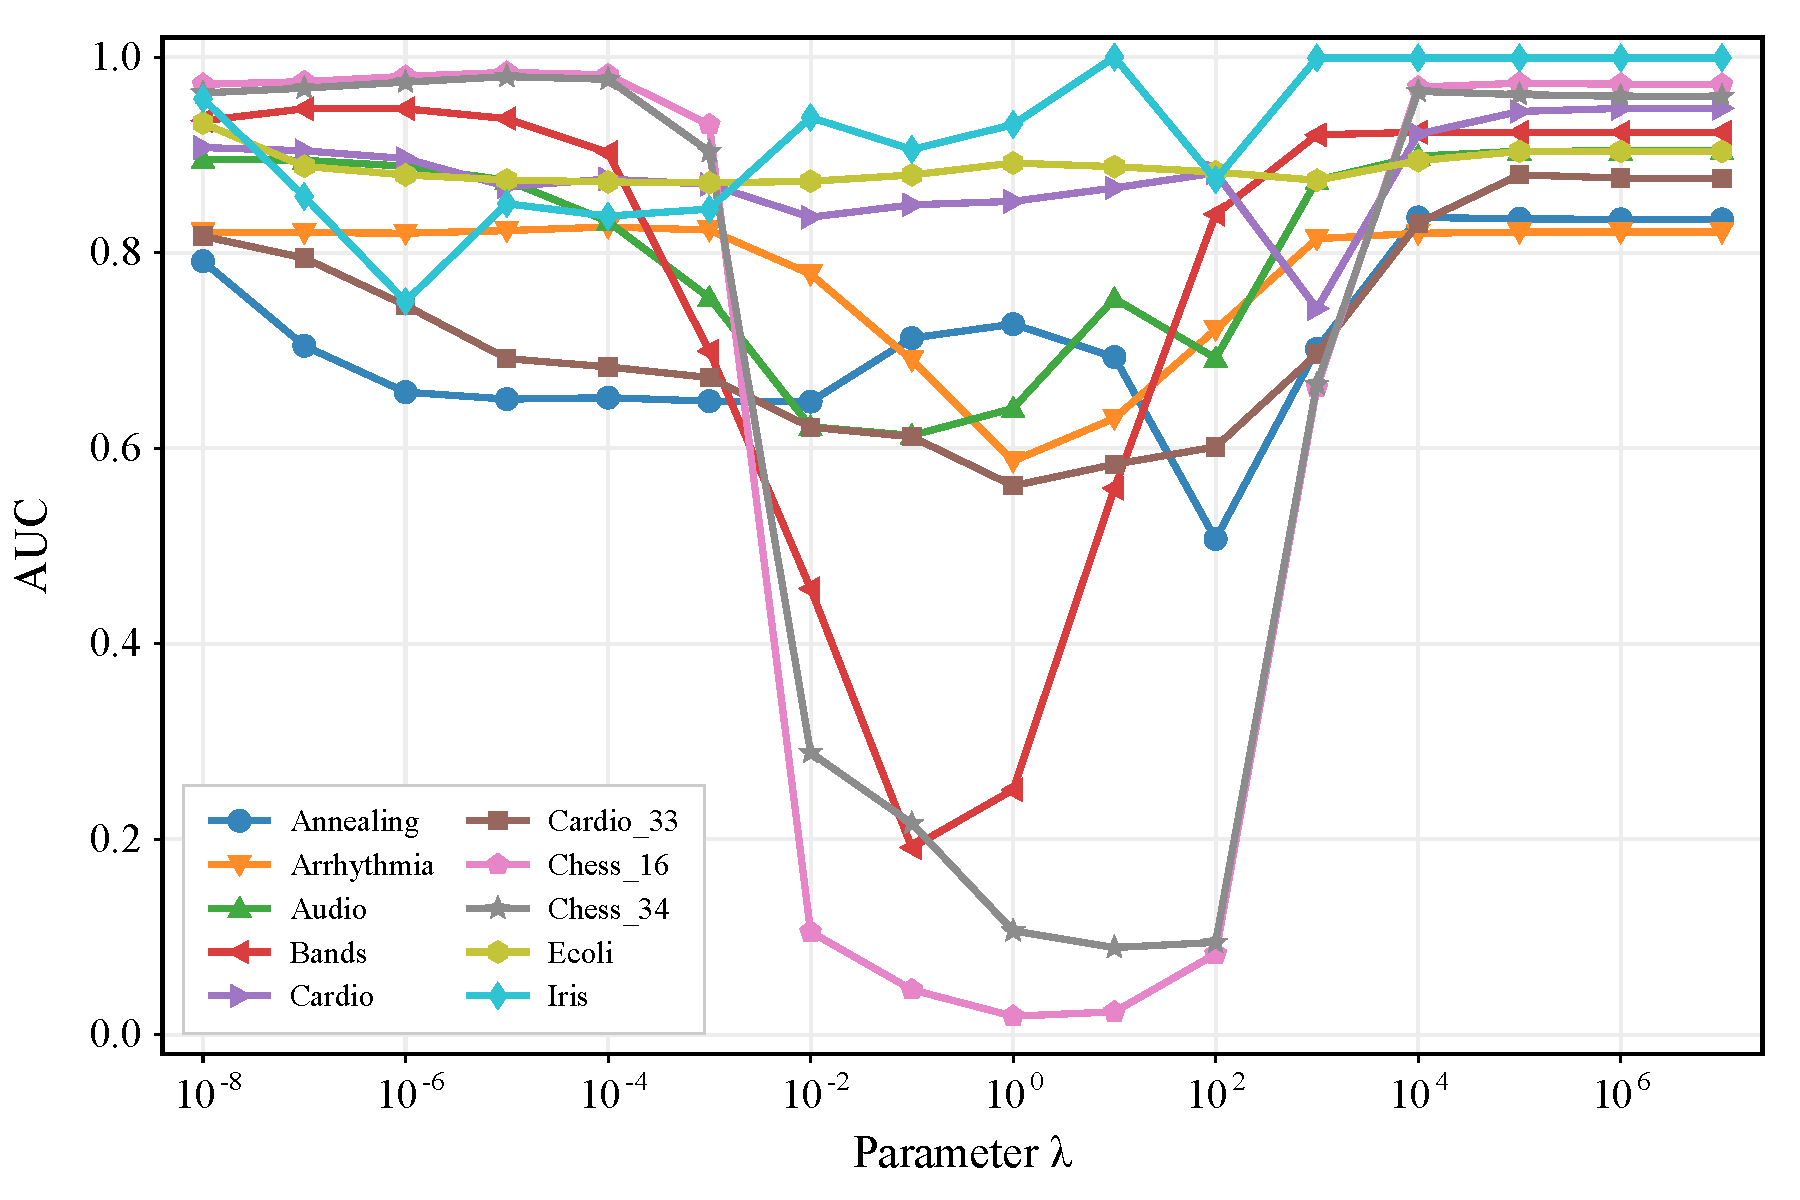
\includegraphics[width=\linewidth]{Figures/KSRA_lambda_Part1.pdf}\\
        \small (a) Datasets 1--10
        \label{fig:lambda_part1}
    \end{minipage}\hspace{8pt}%          
    \begin{minipage}[b]{0.40\textwidth}
        \centering
        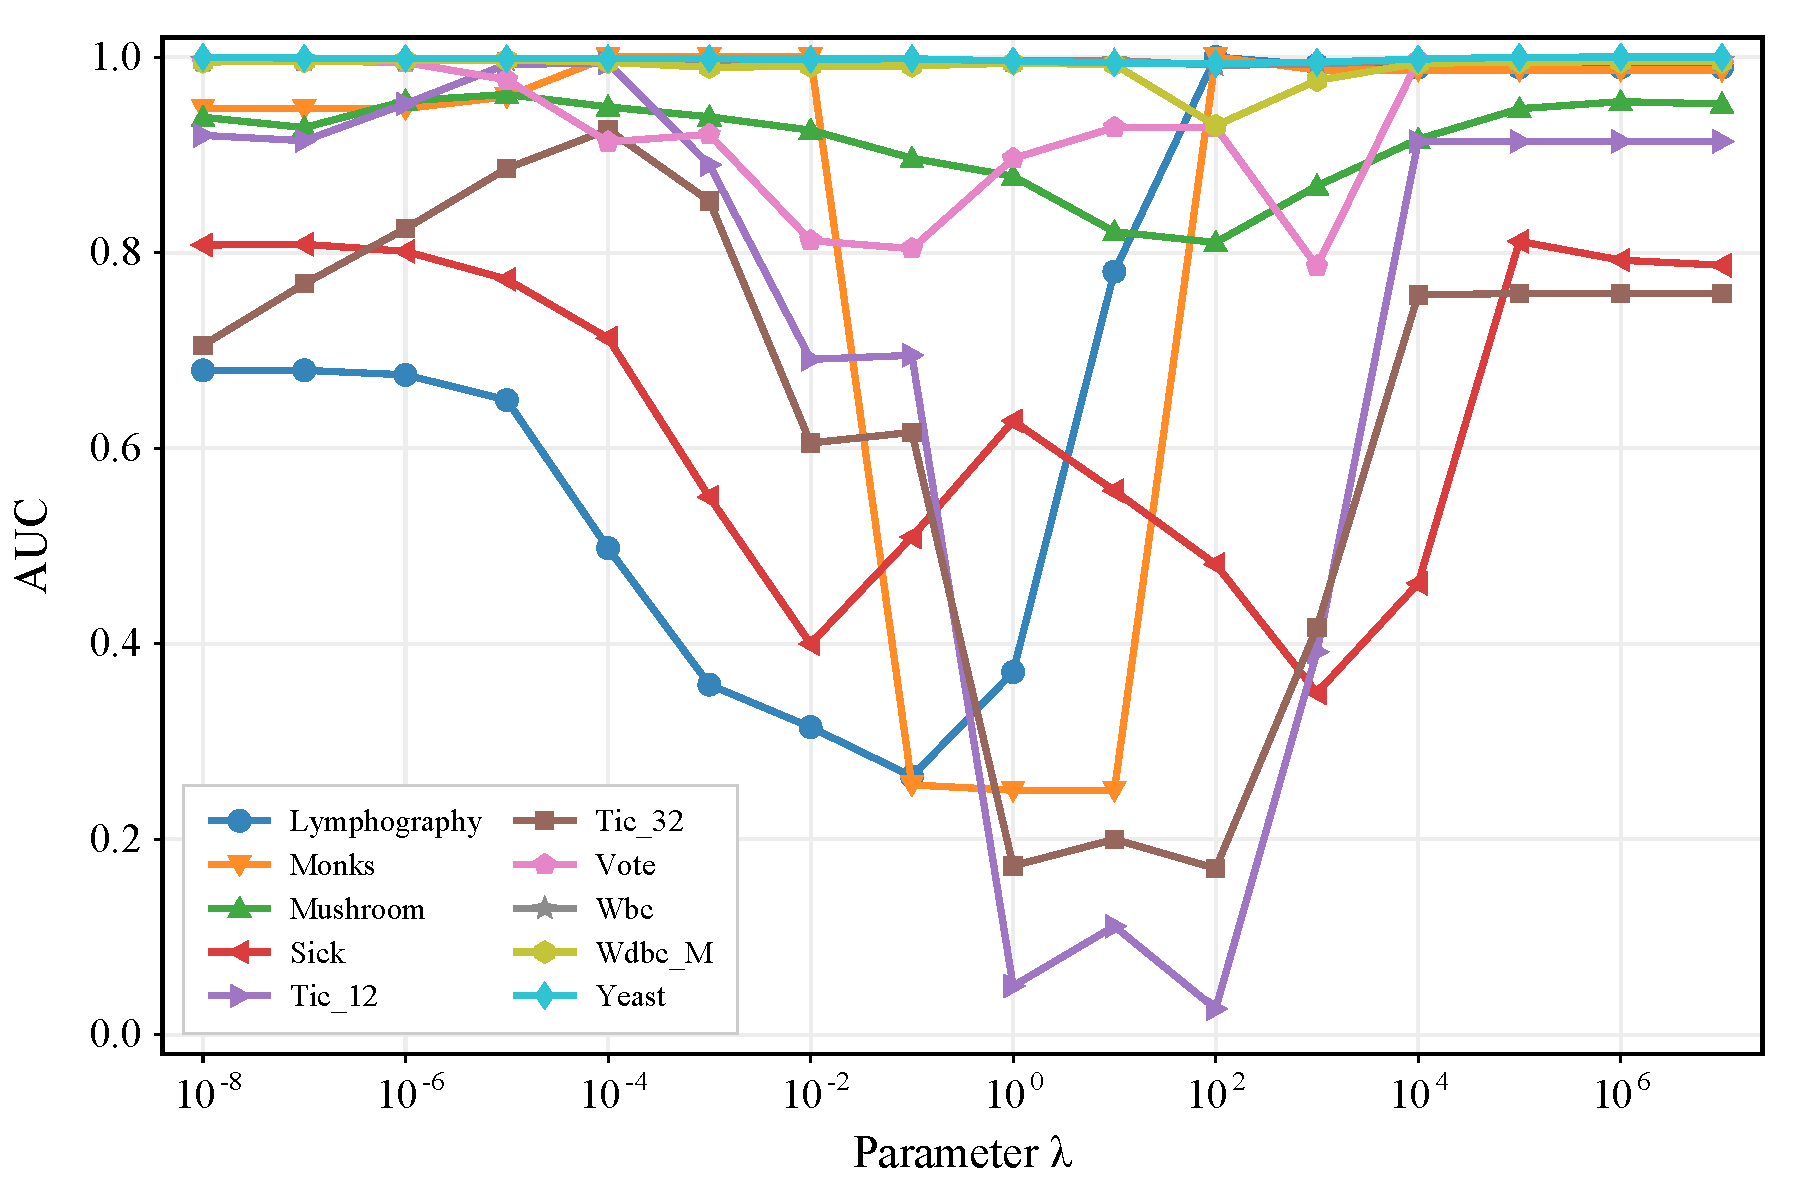
\includegraphics[width=\linewidth]{Figures/KSRA_lambda_Part2.pdf}\\
        \small (b) Datasets 11--20
        \label{fig:lambda_part2}
    \end{minipage}

    \vspace{10pt}

    % ===== 第二行 =====
    \begin{minipage}[b]{0.40\textwidth}
        \centering
        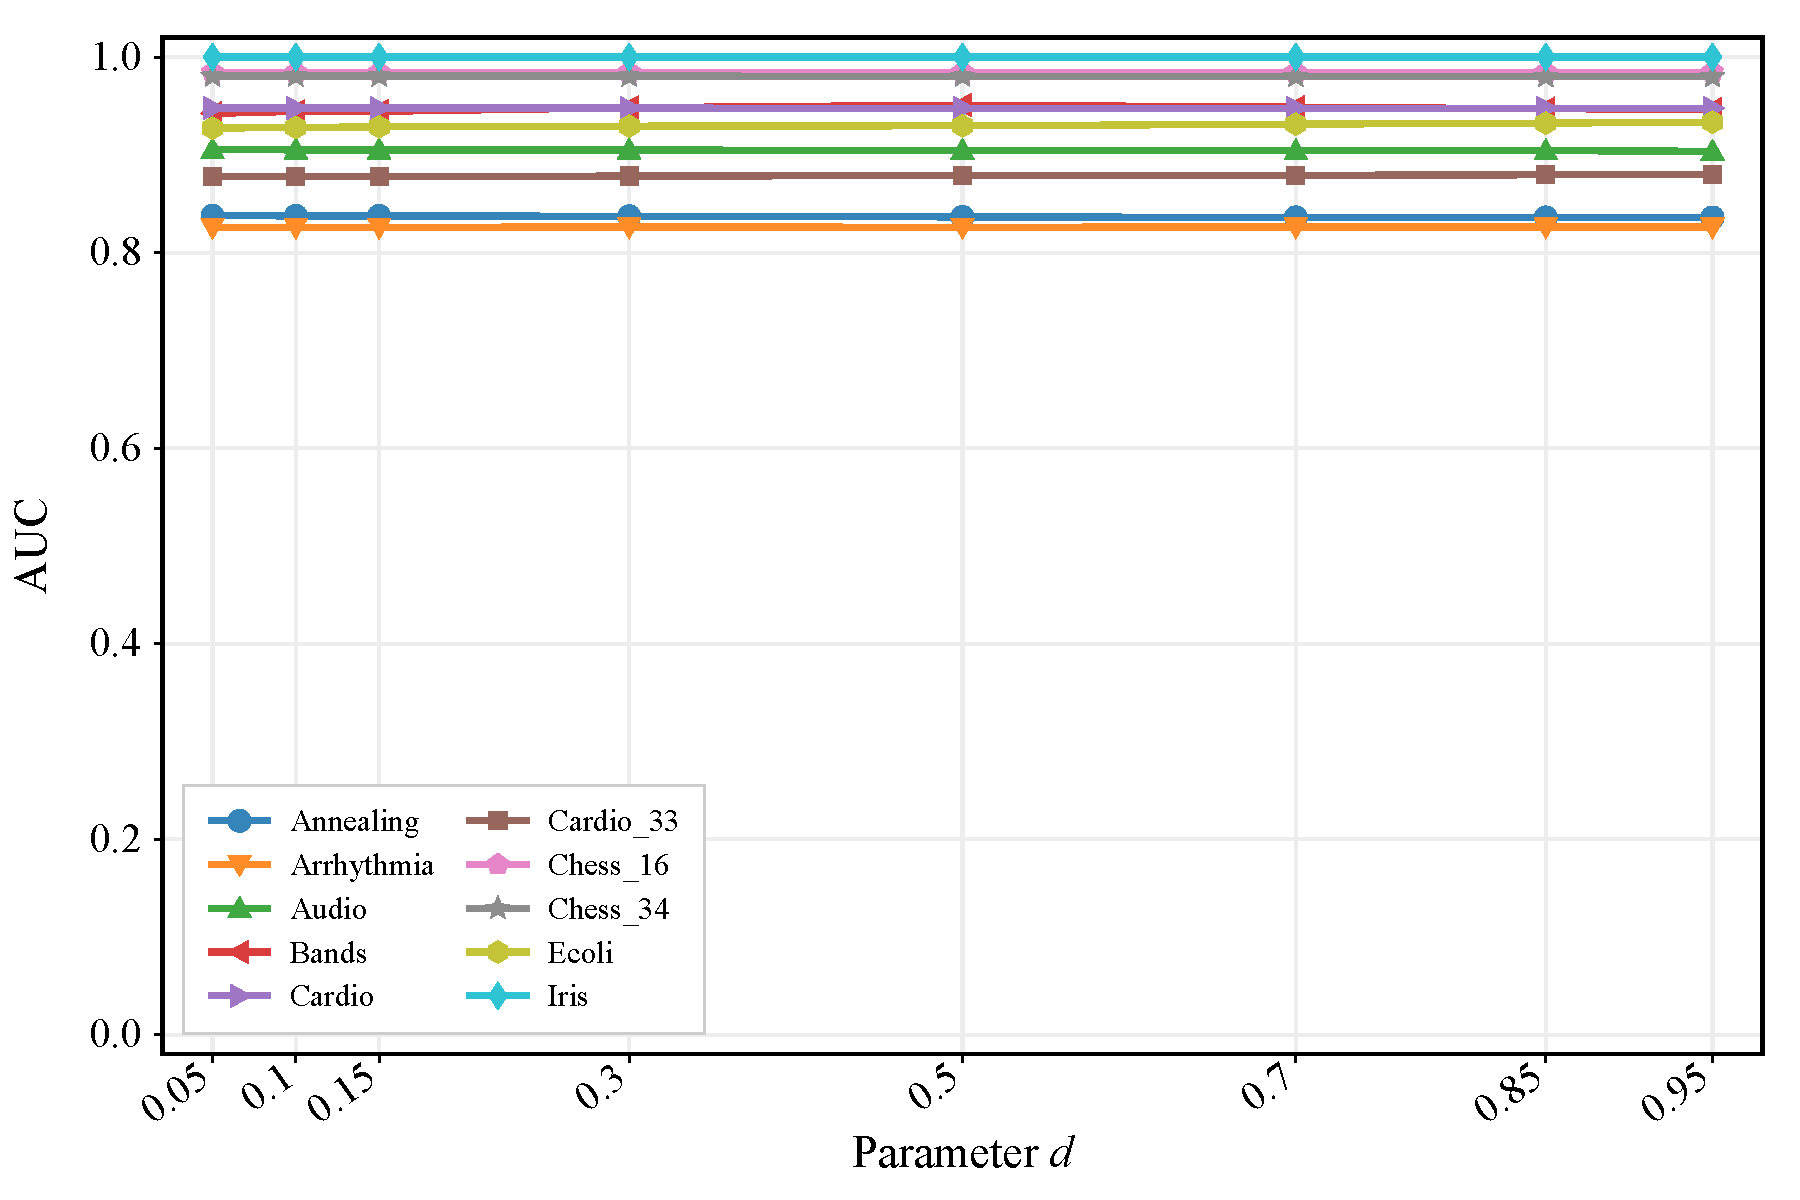
\includegraphics[width=\linewidth]{Figures/KSRA_d_Part1.pdf}\\
        \small (c) Datasets 1--10
        \label{fig:d_part1}
    \end{minipage}\hspace{8pt}%
    \begin{minipage}[b]{0.40\textwidth}
        \centering
        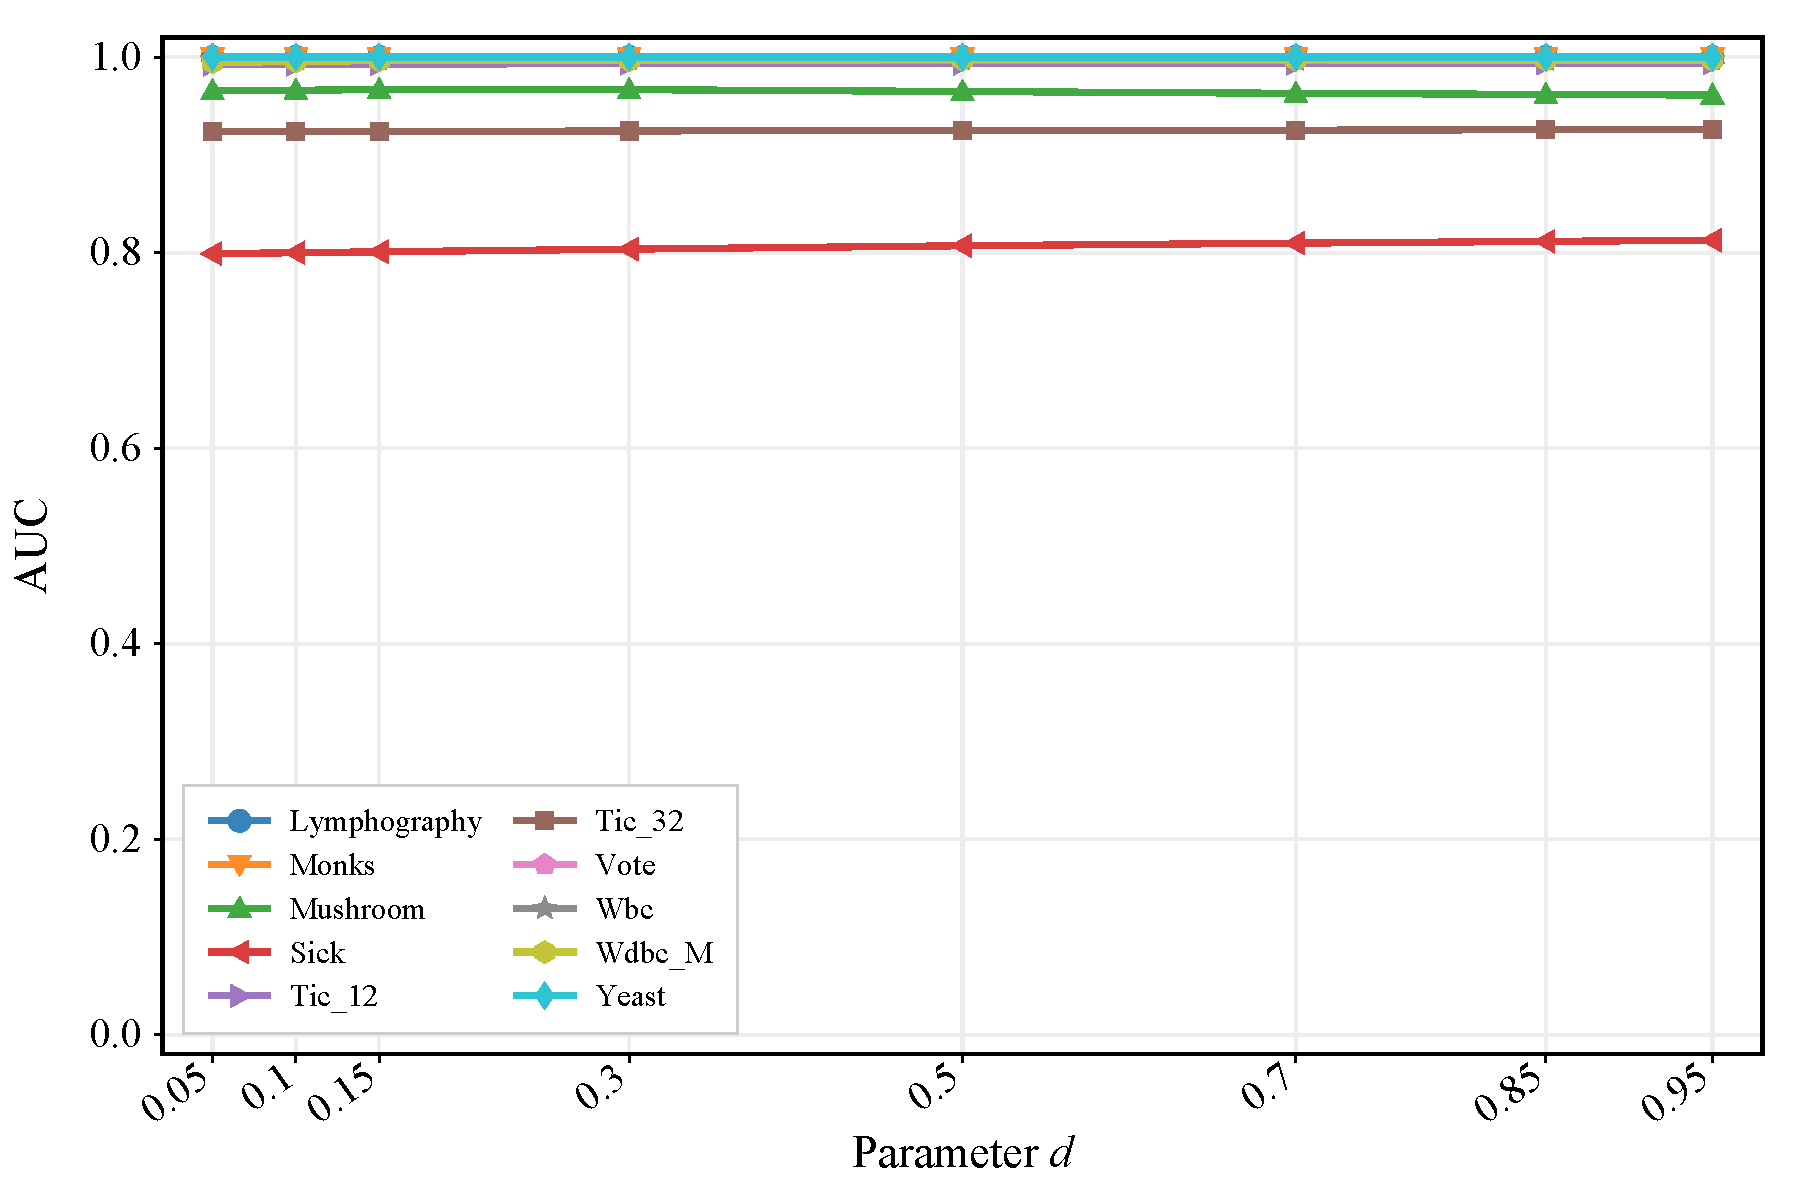
\includegraphics[width=\linewidth]{Figures/KSRA_d_Part2.pdf}\\
        \small (d) Datasets 11--20
        \label{fig:d_part2}
    \end{minipage}

    \vspace{10pt}

    % ===== 第三行 =====
    \begin{minipage}[b]{0.40\textwidth}
        \centering
        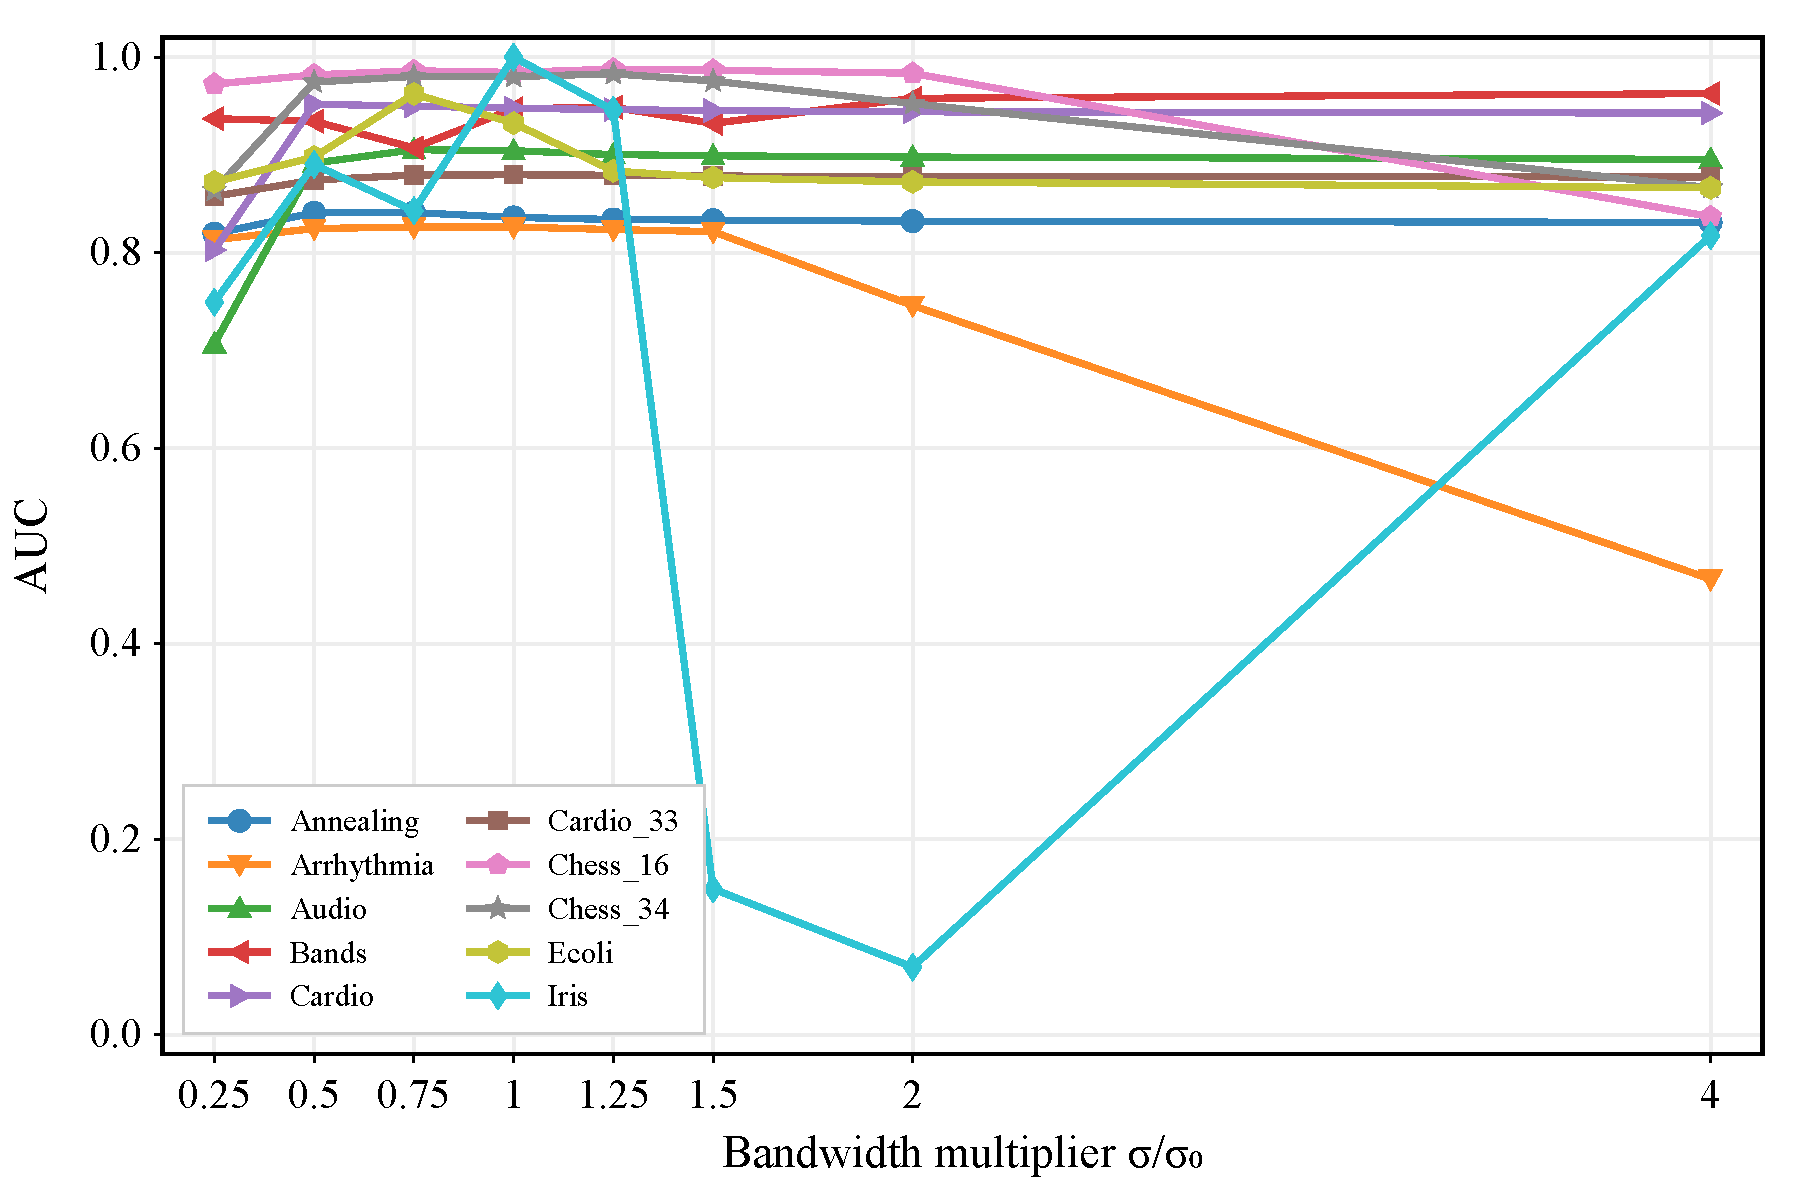
\includegraphics[width=\linewidth]{Figures/KSRA_sigma_Part1.pdf}\\
        \small (e) Datasets 1--10
        \label{fig:sigma_part1}
    \end{minipage}\hspace{8pt}%
    \begin{minipage}[b]{0.40\textwidth}
        \centering
        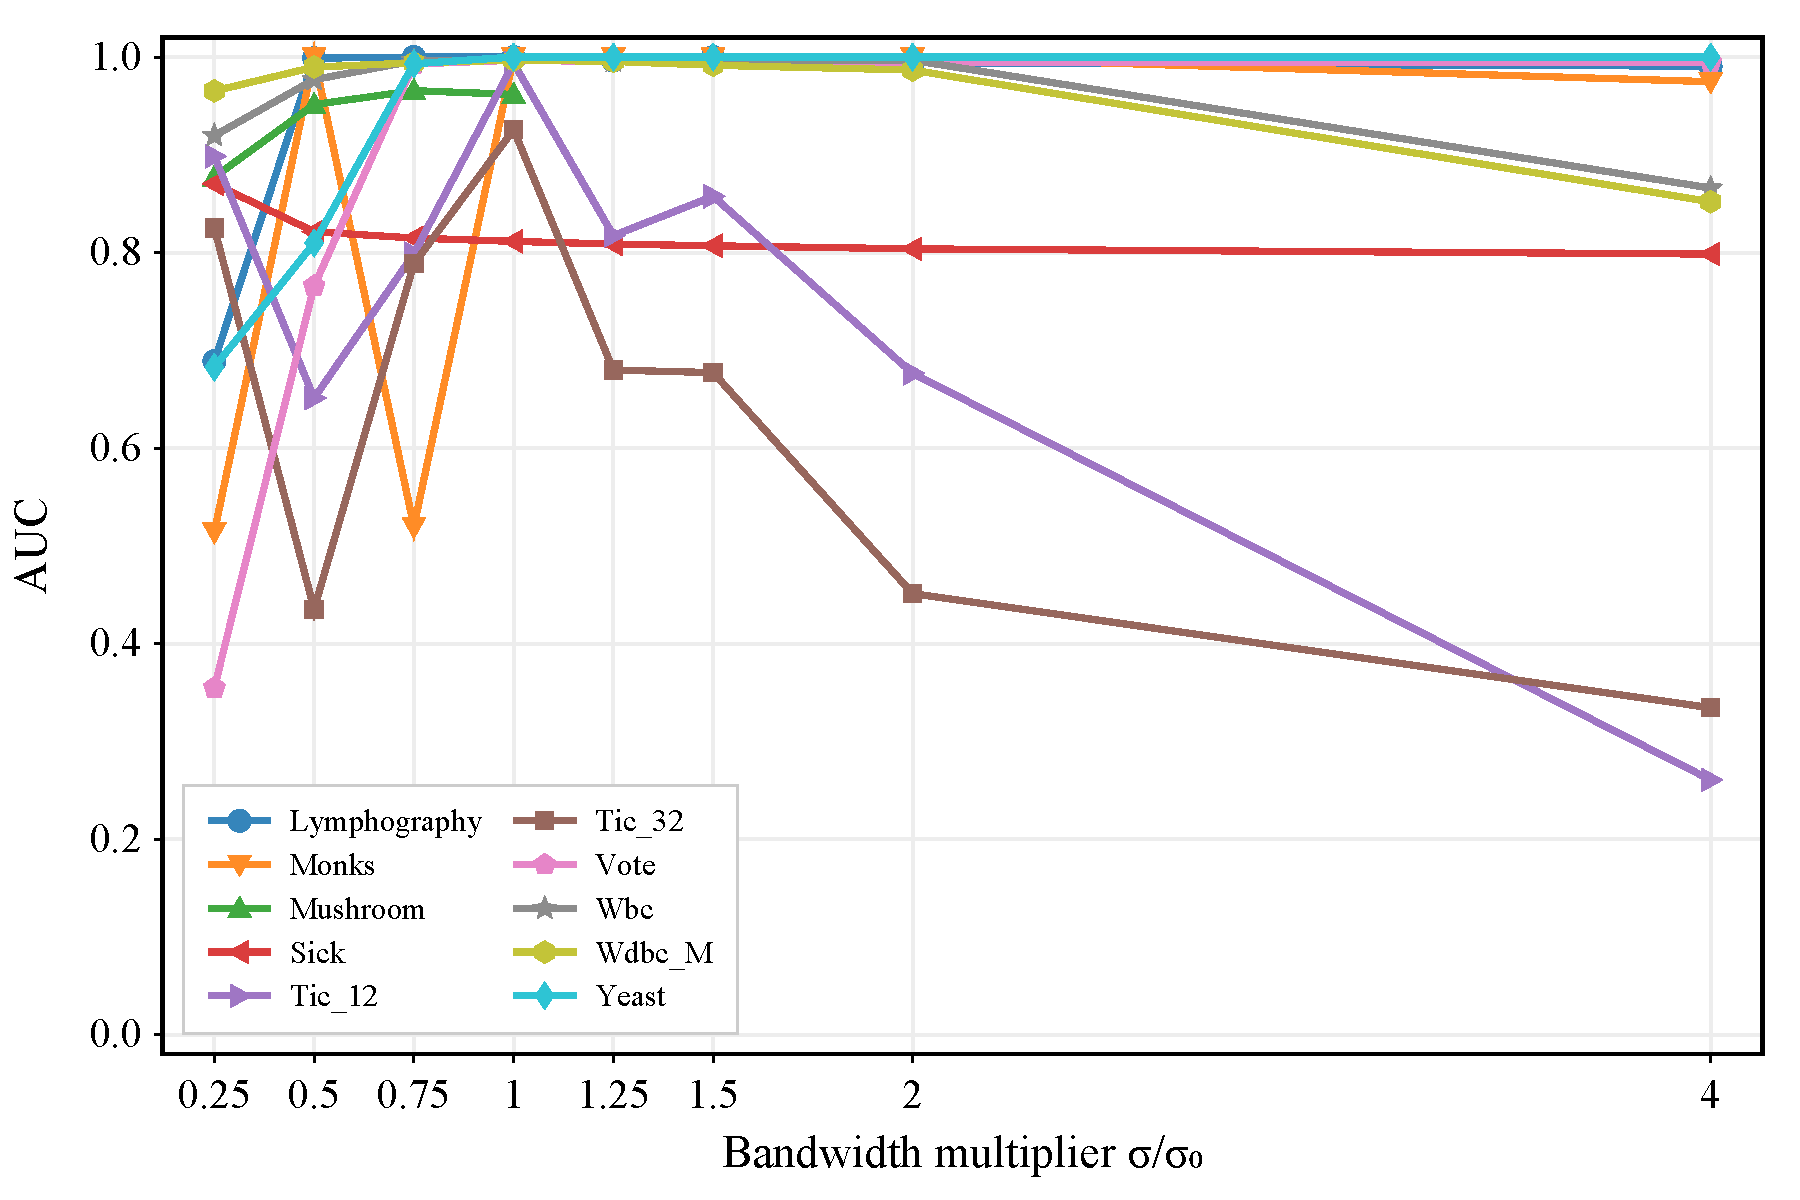
\includegraphics[width=\linewidth]{Figures/KSRA_sigma_Part2.pdf}\\
        \small (f) Datasets 11--20
        \label{fig:sigma_part2}
    \end{minipage}

    \caption{Sensitivity of KSRA to the regularization parameter $\lambda$, restart weight $d$, and kernel bandwidth multiplier $\sigma/\sigma_0$ across 20 benchmark datasets.}
    \label{fig:parameters_sensitivity}
\end{figure*}


\subsection{Ablation Experiments}

To examine the contribution of individual components, we construct three ablation variants of KSRA$_2$, replacing one component at a time. In w/o Hybrid Kernel, we replace the mixed-type kernel with a Gaussian RBF kernel based on Euclidean distances over the prepared features. In w/o Self-Representation, we use the hybrid kernel matrix directly as the graph affinity matrix. In w/o Random Walk, we replace stationary visiting probabilities with weighted degrees computed from the same affinity graph. In this last variant, low degree indicates greater structural abnormality, and we retain min–max normalization and multiplicative score fusion. Whenever self-representation is retained, both the reconstruction loss and coefficient penalty use squared Frobenius norms.

We evaluate all variants on the same 20 benchmark datasets. The bandwidth is the mean off-diagonal distance under the corresponding distance measure, and the restart weight is 0.85 whenever random-walk propagation is retained. For methods with self-representation, we independently select $\lambda$ from $\{10^{-8},10^{-7},\ldots,10^{7}\}$ by the highest evaluation ROC-AUC on each dataset. We also evaluate the ablations with $\lambda$ fixed to the value selected for the full model on each dataset. The variant without self-representation has no $\lambda$, so its two averages coincide. Table~\ref{tab:ablation_study} reports both averages. The Difference column gives the change in mean AUC relative to full KSRA$_2$ under independent tuning, expressed in percentage points.

\begin{enumerate}[\indent (1)]
    \item Replacing the hybrid kernel reduces the mean AUC from 0.9460 to 0.9181 after independent tuning, a decrease of 2.80 percentage points. The largest decreases occur on Bands (0.338 AUC units) and Audio (0.113). The mean AUC drops to 0.8196 when $\lambda$ is held fixed, showing that retuning recovers part of the performance lost after the kernel replacement.

    \item Using the hybrid kernel directly as the affinity matrix reduces the mean AUC to 0.9250, a decrease of 2.10 percentage points. The full model achieves higher AUC on 19 datasets and ties on one. The largest decreases occur on Tic\_32 and Tic\_12, supporting the contribution of learned self-representation on these benchmarks.

    \item Replacing random-walk propagation with weighted-degree scoring yields a mean AUC of 0.9459 after independent tuning and 0.9446 at the full-model $\lambda$. The full model achieves higher AUC on 10 datasets, ties on four, and trails on six under either setting. The mean differences are 0.02 and 0.14 percentage points, respectively, indicating similar average ROC-AUC for the two scoring mechanisms on these benchmarks.
\end{enumerate}

To assess the value of multiplicative fusion in Eq.~(\ref{fuse_outlier_score}), we compare three scoring rules on all 20 benchmark datasets: the isolation weights $\boldsymbol{w}$ from Eq.~(\ref{initial_anomaly_belief}), the normalized random-walk structural scores $\hat{\boldsymbol{s}}_{rw}$, and their element-wise product. For each dataset, the three rules use the same score components computed under the parameter setting selected for the full KSRA$_2$ model. The product achieves a mean ROC-AUC of 0.9460, compared with 0.8461 for the structural scores alone and 0.9255 for the isolation weights alone. It improves on the isolation weights on 19 datasets and ties on one. Relative to the structural scores, it improves on 11 datasets, ties on two, and scores lower on seven. These results support the complementary role of the two components across the benchmark suite, with the benefit of fusion varying by dataset. 

We also evaluated weighted arithmetic fusion, $\beta\hat{\boldsymbol{s}}_{rw}+(1-\beta)\boldsymbol{w}$, using the same score components and applying each candidate weight $\beta\in\{0,0.1,\ldots,1\}$ across all 20 datasets. Equal weighting yielded a mean ROC-AUC of 0.9214. The highest mean among the tested weights was 0.9457 at $\beta=0.2$, close to the 0.9460 achieved by multiplicative fusion. On these benchmarks, multiplicative fusion achieved comparable performance to the best tested weighted average without introducing an additional mixing weight. Uniform restart assigns equal restart input to all nodes, while $\boldsymbol{w}$ enters at the final scoring stage. Using normalized $\boldsymbol w$ as the restart distribution would instead bias the walk toward nodes with larger isolation weights and change the structural scores themselves.

\begin{table*}[!ht]
  \centering
  \caption{Ablation study results of KSRA in terms of average AUC across the 20 benchmark datasets.}
  \label{tab:ablation_study}
  \resizebox{\textwidth}{!}{%
    \begin{tabular}{lccccccccccccccccccccccc}
      \toprule
      Method & Annealing & Arrhythmia & Audio & Bands & Cardio & Cardio\_33 & Chess\_16 & Chess\_34 & Ecoli & Iris & Lymphography & Monks & Mushroom & Sick & Tic\_12 & Tic\_32 & Vote & Wbc & Wdbc\_M & Yeast & Average & Difference & Average (fixed $\lambda$) \\
      \midrule
      KSRA & 0.836 & \textbf{0.826} & 0.904 & \textbf{0.947} & \textbf{0.948} & \textbf{0.880} & 0.984 & 0.980 & \textbf{0.932} & \textbf{1.000} & \textbf{1.000} & \textbf{1.000} & 0.962 & \textbf{0.811} & 0.994 & 0.926 & \textbf{0.997} & \textbf{0.997} & \textbf{0.997} & \textbf{1.000} & 0.9460 & 0.00 & 0.9460 \\
      w/o Hybrid Kernel & 0.754 & 0.809 & 0.792 & 0.610 & \textbf{0.948} & \textbf{0.880} & \textbf{0.986} & \textbf{0.983} & \textbf{0.932} & \textbf{1.000} & 0.992 & \textbf{1.000} & 0.934 & 0.779 & \textbf{0.997} & \textbf{0.978} & 0.995 & \textbf{0.997} & \textbf{0.997} & \textbf{1.000} & 0.9181 & -2.80 & 0.8196 \\
      w/o Self-Representation & 0.836 & 0.819 & 0.891 & 0.925 & 0.944 & 0.878 & 0.973 & 0.962 & 0.894 & 0.999 & 0.992 & 0.987 & 0.953 & 0.797 & 0.914 & 0.758 & \textbf{0.997} & 0.995 & 0.993 & 0.995 & 0.9250 & -2.10 & 0.9250 \\
      w/o Random Walk & \textbf{0.838} & 0.825 & \textbf{0.905} & 0.941 & \textbf{0.948} & 0.878 & 0.984 & 0.981 & 0.924 & \textbf{1.000} & \textbf{1.000} & \textbf{1.000} & \textbf{0.979} & 0.809 & 0.993 & 0.924 & \textbf{0.997} & \textbf{0.997} & 0.995 & \textbf{1.000} & 0.9459 & -0.02 & 0.9446 \\
      \bottomrule
    \end{tabular}%
  }
  \par\vspace{2pt}
  \parbox{\textwidth}{\footnotesize\textit{Note:} The dataset columns and Average use the highest observed AUC for each method. Difference is the change from full KSRA$_2$ in percentage points. Average (fixed $\lambda$) uses each dataset\textquotesingle s full-model $\lambda$ for all methods with self-representation. The variant without self-representation has no $\lambda$. Means and differences are calculated before rounding.}
\end{table*}



\subsection{Distance Concentration and Kernel-Profile Representation}

To examine changes in distances and kernel representations with increasing irrelevant dimensionality, we fixed the sample size at 500, with 20 numerical and 10 categorical base features. We appended 0, 20, 50, 100, 200, and 500 independent irrelevant numerical features. Both structureless data and structured data containing 5\% anomalies were considered, using five data-generation seeds per setting. Kernel bandwidths were determined by the mean off-diagonal distance.

Fig.\ref{fig:distance_concentration_geometry}(a) and (b) show the distance coefficient of variation (CV) for the two scenarios. Here, kernel-profile distance denotes the Euclidean distance between kernel-matrix rows, characterizing the representations supplied to self-representation learning. Higher CV indicates greater relative distance dispersion. Fig.\ref{fig:distance_concentration_geometry}(c) additionally reports the standardized class-separation measure:
\begin{equation*}
    G=
\frac{\mu_{\mathrm{NA}}-\mu_{\mathrm{NN}}}
{\sqrt{(s_{\mathrm{NA}}^2+s_{\mathrm{NN}}^2)/2}},
\end{equation*}
where NA and NN denote normal-anomaly and normal-normal sample pairs, respectively, and $\mu$ and $s$ are the corresponding distance means and standard deviations. Larger positive values indicate clearer distance separation between the two pair types. Curves report means and standard deviations across five repetitions. The measure $G$ is descriptive; overlapping sample pairs are not treated as independent statistical observations.

\begin{enumerate}
    \item Original distances exhibit increasing concentration as irrelevant dimensions are added. Distance CV decreases in both scenarios. For structured data, increasing the total dimensionality from 30 to 530 reduces the mixed-distance CV from 0.3181 to 0.0350, indicating diminished relative distance differences.

    \item Kernel profiles retain greater relative distance variation. At 530 dimensions, hybrid-kernel profiles achieve distance CV values of 0.0514 and 0.1842 on structureless and structured data, respectively, compared with 0.0276 and 0.0350 for the corresponding original mixed distances. At 530 dimensions, distances between hybrid-kernel profiles exhibit greater relative dispersion than the original mixed distances in both synthetic scenarios.

    \item The greater relative dispersion is accompanied by observable class-separation information. On structured data at 530 dimensions, the hybrid-kernel profiles achieve a standardized separation of 3.5860, exceeding the original mixed-distance value of 2.3121. The standardized separation for hybrid-kernel profiles decreases from 11.1165 at 30 dimensions to 3.5860 at 530 dimensions. At 530 dimensions, Euclidean-kernel profiles also improve separation over the original Euclidean distances, increasing $G$ from 4.2105 to 5.7022.
\end{enumerate}

Under the tested synthetic conditions, kernel-profile distances retain greater relative dispersion than their corresponding input distances at the highest tested dimensionality. In the structured scenario, they also provide greater descriptive separation between normal–anomaly and normal–normal pairs at that dimensionality. We assess anomaly detection performance separately using ROC-AUC and AP.

\begin{figure*}[t]
    \centering
    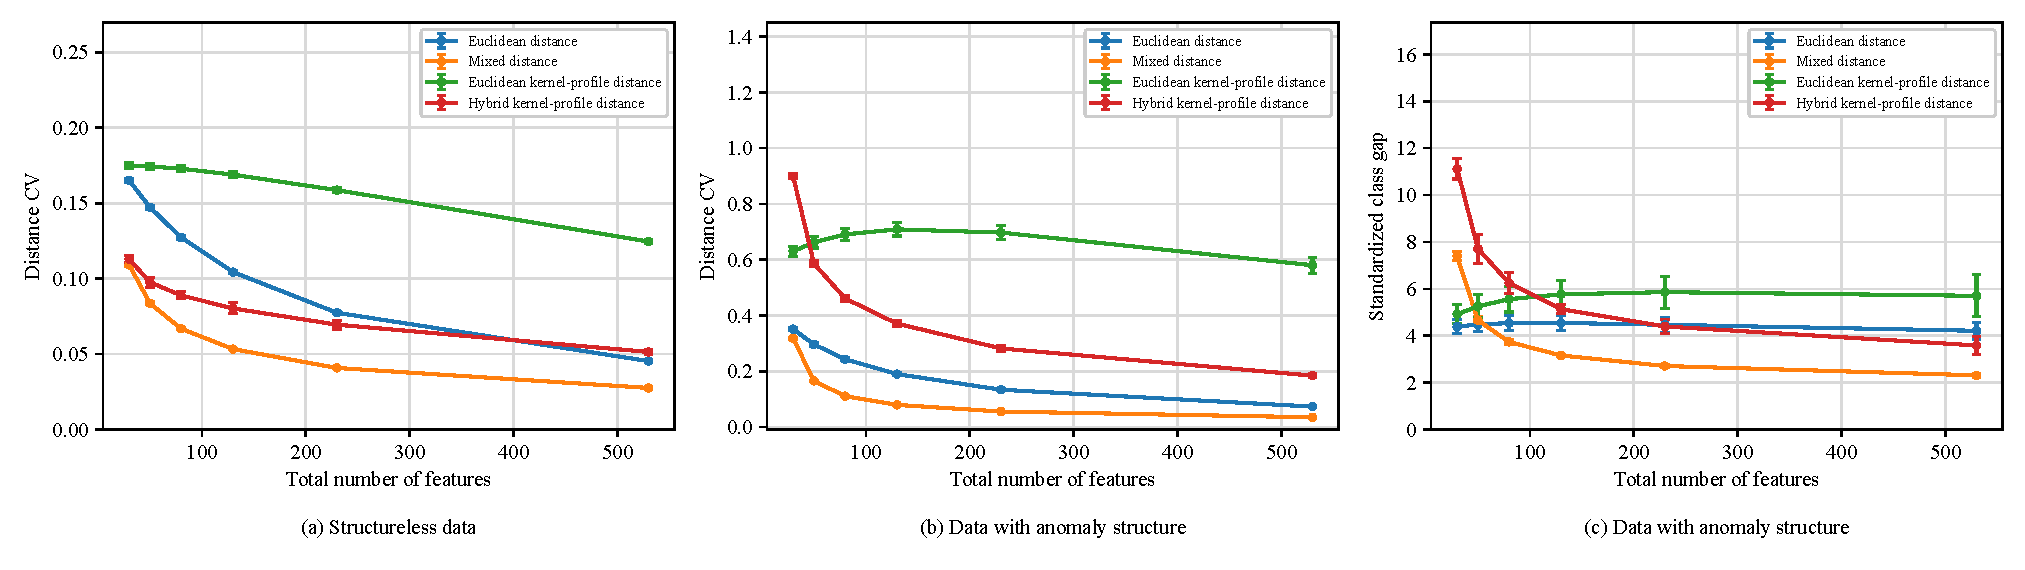
\includegraphics[width=\textwidth]
    {Figures/concentration_geometry_panel.pdf}
    \caption{
        Distance dispersion and class separation as the number of irrelevant features increases. Panels (a) and (b) show the distance coefficient of variation (CV) for structureless data and data with anomaly structure, respectively. Panel (c) shows standardized class separation for data with anomaly structure. Kernel-profile distances are Euclidean distances between rows of the kernel matrix. Error bars indicate standard deviations across five data-generation seeds.
    }
    \label{fig:distance_concentration_geometry}
\end{figure*}


\subsection{Computational Complexity and Scalability Analysis}

Let $n$ denote the number of samples, $m$ the number of features, and $T$ the number of random-walk iterations. Constructing the dense distance and kernel matrices requires $O(n^2m)$ time, and random-walk propagation requires $O(Tn^2)$ time. For self-representation, KSRA$_2$ computes the closed-form solution for the symmetric similarity matrix by dense eigendecomposition and spectral reconstruction, with an $O(n^3)$ cost. KSRA$_1$ and KSRA$_3$ use iteratively reweighted least squares, with costs of $O(L_1n^3)$ and $O(L_3n^3)$, respectively. For KSRA$_4$, $O((L_4+1)n^3)$ is an upper bound for the current ADMM implementation, including dense factorizations and convergence diagnostics. Here, $L_i$ denotes the number of optimization iterations for variant $i$.

All four variants store dense matrices. The current implementation accumulates categorical mismatches one feature at a time within row blocks, requiring $O(Bn)$ temporary space for a block of $B$ rows. The default block size is 256, capped at $n$. Including the input and dense matrices, the overall space complexity is $O(nm+n^2+Bn)=O(nm+n^2)$. The following experiment measures the practical computational cost of KSRA$_2$, the fixed variant used in the main comparison.

We generated synthetic mixed data with 20 numerical features and 10 categorical features, each with four levels. We evaluated KSRA$_2$ at sample sizes of 250, 500, 1000, 2000, 3000, and 4000, with five random seeds per size. We fixed $\lambda=0.01$ and $d=0.85$ and set the bandwidth to the mean off-diagonal mixed distance. Each run used a fresh Windows subprocess with one verified BLAS thread on an Intel Core i5-1035G1 CPU with approximately 16 GiB of RAM and Python 3.8.20. Algorithm timing excluded imports, data generation, warm-up, and file I/O. Peak working set and peak commit were measured over the subprocess lifetime, including runtime overhead. A 2,335 MiB safeguard was applied to both memory measures.

Table~\ref{tab:ksra_scalability} summarizes the computational cost of KSRA$_2$ across the six sample sizes.

\begin{enumerate}[\indent (1)]
    \item All 30 runs completed successfully. The mean execution time increased from 0.021 s at $n=250$ to 10.684 s at $n=3000$ and 27.008 s at $n=4000$. At the largest sample size, the standard deviation across the five runs was 1.754 s.
    
    \item Self-representation accounted for 87.3\% of the mean execution time at $n=3000$ and 89.8\% at $n=4000$. At $n=4000$, graph scoring accounted for 2.2\% of the mean execution time. This stage includes transition-matrix construction, random-walk propagation, and score fusion.

    \item The mean peak working set increased from 55.5 MiB at $n=250$ to 921.9 MiB at $n=4000$. All five runs at $n=4000$ stayed below the 2,335 MiB safeguard. The largest observed peak commit at this size was 930.8 MiB.
\end{enumerate}

The current implementation completed the benchmark at all tested sample sizes up to $n=4000$ within the specified memory safeguard. Blockwise categorical-distance computation limits temporary storage, while the dense representation and graph matrices retain quadratic memory requirements in the number of samples. Dense spectral self-representation remains the dominant runtime cost at the larger tested sizes. Kernel approximation and scalable self-representation solvers are directions for extending the method to larger datasets.

\begin{table*}[!ht]
    \centering
    \caption{Execution time and process peak memory of KSRA$_2$ across six sample sizes. }
    \label{tab:ksra_scalability}
    \begin{tabular}{rcccc}
        \toprule
        Samples ($n$) &
        Completed &
        Execution time (s) &
        Peak working set (MiB) &
        Peak commit (MiB) \\
        \midrule
          250  & 5/5 & $0.021 \pm 0.002$  &  55.5 &  61.3 \\
          500  & 5/5 & $0.094 \pm 0.003$  &  66.7 &  72.5 \\
        1,000  & 5/5 & $0.526 \pm 0.024$  & 109.7 & 115.9 \\
        2,000  & 5/5 & $3.495 \pm 0.051$  & 274.1 & 280.5 \\
        3,000  & 5/5 & $10.684 \pm 0.268$ & 544.3 & 552.5 \\
        4,000  & 5/5 & $27.008 \pm 1.754$ & 921.9 & 930.8 \\
        \bottomrule
    \end{tabular}
\end{table*}





\section{Conclusions}\label{Conclusions}

KSRA learns reconstruction relationships from mixed-attribute similarity profiles and combines structural anomaly evidence with a kernel-derived isolation weight. Across the benchmark suite, KSRA$_2$ ranked second in mean average precision among the fixed methods. The ablations showed lower mean ROC-AUC when the hybrid kernel was replaced with a Euclidean RBF kernel or self-representation was removed, while weighted-degree scoring and random-walk scoring achieved similar mean ROC-AUC.

Two practical limitations remain. The reported benchmark performance depends on evaluation-based hyperparameter selection, and the dense matrices impose quadratic storage requirements in the number of samples. Future work will evaluate label-independent hyperparameter selection and investigate kernel approximations and more scalable self-representation solvers.


%\backmatter

\bmsubsection*{Acknowledgments}
This work was supported by the National Natural Science Foundation of China (62306196 and 12501439) and Sichuan Science and Technology Program (2026NSFSC0783).

\bmsubsection*{Financial Disclosure}

None reported.

\bmsubsection*{Conflicts of Interest}

The authors declare no conflicts of interest.

\bibliography{wileyNJD-Chicago}


\end{document}
